% Format teze zasnovan je na paketu memoir
% http://tug.ctan.org/macros/latex/contrib/memoir/memman.pdf ili
% http://texdoc.net/texmf-dist/doc/latex/memoir/memman.pdf
% 
% Prilikom zadavanja klase memoir, navedenim opcijama se podešava 
% veličina slova (12pt) i jednostrano štampanje (oneside).
% Ove parametre možete menjati samo ako pravite nezvanične verzije
% mastera za privatnu upotrebu (na primer, u b5 varijanti ima smisla 
% smanjiti 
\documentclass[12pt,oneside]{memoir}
\newcommand\tab[1][0.5cm]{\hspace*{#1}} 
% Paket koji definiše sve specifičnosti master rada Matematičkog fakulteta
\usepackage[latinica,biblatex]{matfmaster} 
\usepackage{verbatim}
\usepackage{url}
\usepackage{hyperref}
\newtheorem{primer}{Primer}
\usepackage{enumitem}

\usepackage[latinica]{pangrami}
\usepackage{listings}
\usepackage{color}
 
\definecolor{codegreen}{rgb}{0.6,0,0}
\definecolor{codegray}{rgb}{0.5,0.5,0.5}
\definecolor{codepurple}{rgb}{0.169, 0.169, 0.169}
\definecolor{backcolour}{rgb}{0.95,0.95,0.92}
 
\lstdefinestyle{mystyle}{
    backgroundcolor=\color{backcolour},   
    commentstyle=\color{codegreen},
    keywordstyle=\color{codegreen},
    numberstyle=\tiny\color{codegray},
    stringstyle=\color{codepurple},
    basicstyle=\footnotesize,
    breakatwhitespace=false,         
    breaklines=true,                 
    captionpos=b,                    
    keepspaces=true,                 
    numbers=left,                    
    numbersep=5pt,                  
    showspaces=false,                
    showstringspaces=false,
    showtabs=false,                  
    tabsize=2
}
 
\lstset{style=mystyle}




% Datoteka sa literaturom u BibTex tj. BibLaTeX/Biber formatu
\bib{literatura}

% Ime kandidata na srpskom jeziku (u odabranom pismu)
\autor{Ana Đorđević}
% Naslov teze na srpskom jeziku (u odabranom pismu)
\naslov{Automatsko generisanje test primera uz pomoć statičke analize i rešavača Z3}
% Godina u kojoj je teza predana komisiji
\godina{2018}
% Ime i afilijacija mentora (u odabranom pismu)
\mentor{dr Milena \textsc{Vujošević Janičić}, docent\\ Univerzitet u Beogradu, Matematički fakultet}
% Ime i afilijacija prvog člana komisije (u odabranom pismu)
\komisijaA{dr Filip \textsc{Marić}, vanredni profesor\\ Univerzitet u Beogradu, Matematički fakultet}
% Ime i afilijacija drugog člana komisije (u odabranom pismu)
\komisijaB{dr Milan \textsc{Banković}, docent \\ Univerzitet u Beogradu, Matematički fakultet}
% Ime i afilijacija trećeg člana komisije (opciono)
% \komisijaC{}
% Ime i afilijacija četvrtog člana komisije (opciono)
% \komisijaD{}
% Datum odbrane (odkomentarisati narednu liniju i upisati datum odbrane ako je poznat)
% \datumodbrane{}

% Apstrakt na srpskom jeziku (u odabranom pismu)
\apstr{%
}

% Ključne reči na srpskom jeziku (u odabranom pismu)
\kljucnereci{verifikacija softvera, testiranje softvera, SMT rešavači, Z3 rešavač, automatsko pronalaženje grešaka u programu, računarstvo}
\begin{document}
% ==============================================================================
% Uvodni deo teze
\frontmatter
% ==============================================================================
% Naslovna strana
\naslovna
% Strana sa podacima o mentoru i članovima komisije
\komisija
% Strana sa posvetom (u odabranom pismu)
\posveta{Mami i tati}
% Strana sa podacima o disertaciji na srpskom jeziku
%\apstrakt
% Sadržaj teze
\tableofcontents*

% ==============================================================================
% Glavni deo teze
\mainmatter
% ==============================================================================

% ------------------------------------------------------------------------------
\chapter{Uvod}

Značajan razvoj računarstva i informatike poslednjih decenija uveo je softver u sve segmente života. Razvijeni su brojni softverski sistemi raznovrsnih namena koji se koriste kako za neobavezne tako i za poslovne aktivnosti. Softver je postao neophodan u svim oblastima društva uključujući, između ostalog, privredu, obrazovanje, zdravstvo i medije.

Složenost softverskih sistema neizbežno stvara veći prostor za pravljenje grešaka. U zavisnosti od namene sistema, greške mogu izazvati neprijatnosti ali i katastrofalne
posledice po živote ljudi. Kako bismo izbegli ovakve situacije, neophodno je precizno utvrditi ispravnost razvijenog softvera.

Ispravnost softvera najčešće se utvrđuje njegovim izvršavanjem, tj. testiranjem. Prostor mogućih ulaza programa obično je prevelik pa nije moguće pokretanje i provera programa svim mogućim ulazima. Poželjno je sprovesti testiranje sistema koristeći samo reprezentativni skup ulaznih podataka. Automatizacija procesa generisanja test primera i provera rezultata testiranja posebno je važna jer
olakšava i ubrzava proces testiranja.

Ispravnost softvera je moguće proveravati i bez njegovog izvršavanja, samo na osnovu analize izvornog koda, korišćenjem tehnika statičke analize. Statička analiza
koda može biti manuelna, i podrazumeva ručne provere i preglede koda, ili može biti automatizovana.

U okviru statičke automatizovane provere ispravnosti softvera formiraju se uslovi ispravnosti iskazani formulama u terminima matematičkih teorija  \cite{RigorousSD}. Formirani
uslovi ispravnosti definišu model kojim se opisuje ponašanje programa  \cite{ModelCheck}. Proveravanjem modela, primenom različitih tehnika testiranja pronalaze se greške u
sistemu. Sistemi za statičku analizu koda mogu se koristiti i za automatsko
generisanje test primera.

\subsection{Doprinos rada}

U okviru ovog rada nadograđen je sistem za statičku proveru ispravnosti softvera LAV modulom za automatsko generisanje test primera \cite{LAVTool}. U okviru sistema
LAV, ponašanje programa modeluje se formulama izabrane teorije. Nadogradnja obuhvata prepoznavanje ulaznih vrednosti programa, a zatim izdvajanje odgovarajućih vrednosti iz modela generisanih od strane alata LAV i rešavača Z3. Na osnovu vrednosti izdvojenih iz modela, formira se test primer za koji je potrebno pokrenuti izvršavanje programa i proveriti da li generisani test primer zaista dovodi do greške u softveru.

\subsection{Pregled rada}
Nastavak rada organizovan je na sledeći način. U glavi \ref{testiranje} opisan je proces testiranja kao važan deo životnog ciklusa razvoja softvera. Navedene su vrste i strategije testiranja uključujući strategiju crne, bele i sive kutije. Opisani su načini izvršavanja i generisanja test primera. Navedeni su neki od alata za automatsko generisanje test primera. Glava \ref{resavac} daje motivaciju za korišćenje rešavača tokom statičke provere ispravnosti softvera. Opisuju se osnove rešavača Z3 navođenjem podržanih teorija. Dat je pregled najvažnijih tipova i struktura podataka. Opisana su dva formata za komunikaciju sa Z3 rešavačem korišćenjem SMT-LIB standarda i C++ interfejsa i njihova upotreba kroz primere. U glavi \ref{implementacija} opisan je detaljno problem kojim se rad bavi i predloženo rešenje. Opisana je statička provera ispravnosti softvera uključujući tehnike statičke analize. Dat je pregled alata za statičku proveru ispravnosti programa LAV kao i osvrt na dodatu funkcionalnost. Opisana je integracija koda u postojeće klase i module kao i implementacija novih klasa sa ciljem automatskog generisanja test primera. U glavi \ref{zakljucak} izneti su osnovni zaključci ovog rada.


%Dat je opis arhitekture i implementacije modula za automatsko generisanje test primera upotrebom statičke analize i rešavača Z3 integrisanog u sistem LAV. 

% ------------------------------------------------------------------------------


% ------------------------------------------------------------------------------
\chapter{Testiranje} \label{testiranje}

Testiranje predstavlja važan deo životnog ciklusa razvoja softvera. 
Softver se implementira prema zahtevima korisnika sa ciljem rešavanja realnog problema ili kreiranja potrebne funkcionalnosti. Nakon implementacije, softver može u manjoj ili većoj meri odgovarati zahtevima. Svako ponašanje softvera koje se ne slaže sa zahtevima predstavlja grešku koju je potrebno detektovati i eliminisati. 
\par
Testiranje predstavlja proveru da li je softver implementiran u skladu sa korisničkim zahtevima. Pored proveravanja samog softvera, testiranje uključuje proveravanje svih pratećih komponenti i karakteristika. 
\par 
Sa porastom složenosti projekta, raste i značaj testiranja i provera celokupnog softverskog sistema kako bi se izbegli ishodi koji mogu da unište ceo projekat. 
S obzirom da se greške ne mogu izbeći, potrebno ih je što je moguće ranije otkriti kako bi njihovo otklanjanje bilo brže i jeftinije. Zbog prednosti koje se ostvaruju, najzastupljenije i trenutno najpopularnije metodologije razvoja softvera promovišu paralelnu implementaciju i pisanje testova za svaku od celina koja se razvija u okviru softverskog sistema \cite{AgileDevelopment}. Pre isporučivanja softvera, neophodno je da uspešno prođu testovi za svaku od celina sistema.
\par 

U delu \ref{broj1} opisane su faze i aktivnosti koje se primenjuju tokom procesa testiranja. U delu \ref{broj2} opisane su vrste testiranja softverskog sistema. U delu \ref{broj3} opisane su strategije testiranja uključujući strategiju crne, bele i sive kutije. Načini izvršavanja testova opisani su u delu \ref{broj4}. Načini generisanja testova opisani su u delu \ref{broj5}. U delu \ref{broj5} opisane su i neke od tehnika i alata za automatsko generisanje test primera korišćenjem strategija crne, bele i sive kutije. 
\section{Testiranje u procesu razvoja softvera} \label{broj1}
\par 
Testiranje softvera se u opštem slučaju sastoji od četiri faze pri čemu svaka faza obuhvata veliki broj aktivnosti. Proces testiranja sastoji se od faza planiranja, dizajniranja, izvršavanja i evaluacije testova \cite{ImportanceOfTesting}.
\par
Planiranje (eng. \textit{Test planning}) predstavlja pripremu za ceo proces testiranja i uključuje definisanje zadataka koje je potrebno sprovesti kao i način njihovog izvršavanja. Tokom ove faze, definišu se vrste testova koje će biti sprovedene, metode testiranja, strategije kao i kriterijum završetka. Rezultat planiranja predstavlja skup dokumenata koji sadrže opštiji pogled na sistem koji će se testirati, aktivnosti koje će biti izvršene kao i alate koji će biti korišćeni.
\par 
Tokom faze dizajniranja testova (eng. \textit{Test design}), vrši se detaljna specifikacija načina na koje će se aktivnosti predviđene planom izvršiti. Pored toga, kreiraju se i precizna uputstva kako će se vršiti testiranje sistema. Tokom ove faze, analizira se sistem koji će biti testiran. Rezultat faze dizajniranja je skup test slučajeva i test procedura koja će biti korišćene u fazi izvršavanja testova.
\par
Izvršavanje testova (eng. \textit{Test execution}) se vrši radi provere funkcionalnosti sistema.
To je proces konkretne primene test slučajeva i test procedura formiranih na osnovu plana i dizajna. Izvršavanje testova obuhvata i dodatnu aktivnost praćenja statusa problema. Ova aktivnost podrazumeva eliminaciju prijavljenih problema kao i potvrđivanje da je problem rešen.
\par
Evaluacija testova (eng. \textit{Test evaluation}) predstavlja kreiranje izveštaja kojim se opisuje šta je testirano i potvrđivanje da je implementirani sistem spreman za korišćenje u skladu sa korisničkim zahtevima. Proces evaluacija uključuje i pregled rezultata dobijenih analizom izlaza test slučajeva.   

\section{Vrste testiranja} \label{broj2}

U literaturi se sreću različite podele testiranja softvera. Svaka je nastala kao posledica posmatranja različitih aspekata i pristupa provere softverskog sistema.
Jedan od pristupa odnosi se na testiranje različitih nivoa sistema. Nivoi testiranja mogu biti pojedinačni moduli, grupe modula (vezanih namenom, upotrebom, ponašanjem ili strukturom) ili ceo sistem.
U skladu sa pomenutom podelom, prema nivou testiranja, razlikujemo testove jedinice koda, komponentne, integracione i sistemske testove.
\par
U kasnijim fazama razvoja softvera, kada je testiranje sistema po svim nivoima uspešno završeno, pristupa se izvršavanju istraživačkih testova i testova prihvatljivosti.
\par

Testiranjem jedinice koda (eng. \textit{Unit testing}) proverava se funkcionisanje delova sistema koji se nezavisno mogu testirati \cite{SoftwareUnitTesting}. U zavisnosti od konteksta i programske paradigme, to mogu biti podprogrami ili veće komponente formirane od tesno povezanih jedinica. Ovom vrstom testiranja prolazi se svaki i najmanji deo sistema, pa upravo iz tog razloga ima važnu ulogu prilikom osiguravanja kvaliteta razvijenog softvera. Jedinični testovi definisani su standardom \textit{IEEE Standard for Software Unit Testing} \cite{IEEEStandard}. Cilj jediničnih testova je dokazivanje da komponenta ima predviđenu funkcionalnost. Ukoliko postoje greške u komponenti, one bi trebalo da budu otkrivene u fazi testiranja te komponente. Treba koristiti specijalne slučajeve ulaza, probati granice domena kao i nekorektan ulaz kako bi obezbedili da ne dolazi do pada softverskog sistema pri ovakvim situacijama.
\par
Komponentnim testiranjem (eng. \textit{Component testing}) proveravaju se moduli sastavljeni od više komponenti \cite{ComponentTesting}. Neformalno, komponenta je skup povezanih jedinica koda koje imaju zajednički interfejs prema ostalim komponentama.  Moduli se proveravaju odmah po njihovom kreiranju pri čemu se testiranje može vršiti izolovano od ostatka sistema, u zavisnosti od izabranog modela razvoja. Važno je napomenuti da testiranje jedinica koda obavlja razvojni tim, a testiranje komponenti tim testera. Pored toga, preporuka je da se komponentno testiranje izvrši pre testova integracije koji će biti opisani u nastavku.
\par

Pošto su pojedinačni moduli u sistemu ispravno implementirani, integracionim testiranjem (eng. \textit{Integration testing}) proverava se saradnja između modula koji predstavljaju jednu celinu sistema \cite{IntegrationTesting}. Ispituje se da li su veze između ovih modula dobro definisane i realizovane, tj. da li moduli komuniciraju na način opisan u specifikaciji projekta. 
Integracionim testovima pokazuje se da različiti moduli sistema rade ispravno zajedno. Za izvršavanje integracionih testova, obično se zahteva pristup bazi i hardverskim delovima sistema. Ukoliko je testiranje komponenti uspešno završeno, tokom integracionog testiranja mogu se naći manji propusti u komunikaciji između modula, pri čemu možemo biti sigurni da su funkcionalnosti samih modula ispravno implementirane.
\par
 
Sistemsko testiranje (eng. \textit{System testing}) obuhvata proveravanje sistema kao celine \cite{SystemTesting}. Ispituje se da li je ponašanje sistema u skladu sa specifikacijom zadatom od strane klijenta.
Ova vrsta testiranja stavlja naglasak na nefunkcionalne zahteve sistema kao što su brzina, efikasnost, otpornost na otkaze, uklapanje u okruženje u kojem će se sistem koristiti. 
Testiranje sistema obavlja se u drugačijim uslovima u odnosu na testiranje jedinica koda i testiranje prihvatljivosti. 
U proces testiranja sistema uključuje se ceo razvojni tim pod nadzorom rukovodioca projekta.
Testiranje sistema obuhvata nekoliko koraka pri čemu će u nastavku biti opisano testiranje performansi i instalaciono testiranje. 
\par
Tokom testiranja performansi, izvršavaju se testovi konfiguracije, kapaciteta, kompatibilnosti i bezbednosti kao i regresioni testovi. Testovima konfiguracije ispituje se ponašanje sistema u različitim hardverskim i softverskim okruženjima. 
Različite konfiguracije namenjene su različitim korisnicima sistema.
Ovim testovima proveravaju se sve konfiguracije sistema.
Testovima kapaciteta proverava se ponašanje sistema pri obradama velikih količina podataka. 
Proverava se i ponašanje sistema u slučaju kada skupovi podataka postignu svoje maksimalne kapacitete. 
Testovima kompatibilnosti proverava se način ostvarivanja komunikacije sistema sa drugim spoljnim sistemima.
Ovim testovima se proverava i da li je korisnički interfejs implementiran u skladu sa zahtevima klijenta. 
Svakako, pri testiranju važna karakteristika je bezbednost sistema.
Testovima bezbednosti proverava se da li su određene funkcionalnosti dostupne isključivo onim korisnicima kojima su namenjene. Proveravaju se i dostupnost, integritet i poverljivost svih skupova podataka. 
Regresiono testiranje podrazumeva primenu jednom napisanog test primera nekoliko puta za testiranje istog softvera. 
To se obično radi posle izmena u razvoju sistema, da bi se utvrdilo da nije došlo do lošeg rada nekih funkcija koje nisu bile obuhvaćene izmenama. 
Regresioni testovi garantuju da su performanse novog sistema barem jednake performansama starog. 

\par
Poslednja faza sistemskog testiranja je instalaciono testiranje.
Ova vrsta testiranja izvodi se instaliranjem softvera na klijentskoj mašini.
Prilikom instaliranja, sistem se konfiguriše u skladu sa okruženjem.
Ukoliko je potrebno, sistem se povezuje sa spoljnim uređajima i sa njima uspostavlja komunikaciju. 
Instalacioni testovi se izvršavaju u saradnji sa korisnicima. Ispituje se da li uslovi na klijentskoj mašini i okruženju negativno utiču na neke funkcionalne ili nefunkcionalne osobine sistema. 
Kada rezultati testiranja zadovoljavaju potrebe klijenta, testiranje se prekida i sistem se formalno isporučuje.
\par


Tokom istraživačkog testiranja (eng. \textit{Exploratory testing}) testeri pronalaze i proveravaju druge eventualne pravce korišćenja softverskog sistema \cite{ExploratoryTesting}. Na taj način podstiče se povećanje kreativnosti testera. Ova vrsta testiranja obuhvata aktivnosti prepoznavanja, kreiranja i izvršavanja novih test slučajeva. Istraživačko testiranje uglavnom ima smisla kada je aplikacija u svom finalnom obliku, kada tester može videti i druge alternativne pravce korišćenja sistema koji ranije nisu mogli biti predmet testiranja. Ukoliko se ova faza testiranja preskoči, postoji opasnost da neke funkcionalnosti sistema ne budu pokrivene testovima.
\par 


Testovi prihvatljivosti (eng. \textit{Acceptance testing}) 
treba da omoguće klijentima i korisnicima da se sami uvere da je napravljeni softver u skladu sa njihovim potrebama i očekivanjima \cite{AcceptanceTesting}.
Ovu vrstu testiranja izvode i procenjuju korisnici, a razvojni tim im pruža pomoć oko tehničkih pitanja, ukoliko za tim ima potrebe.
Klijent može da proceni sistem na tri načina: referentnim testiranjem, pilot testiranjem i paralelnim testiranjem. Kod referentnog testiranja, klijent generiše test slučajeve koji predstavljaju uobičajne uslove u kojima sistem treba da radi. Ove testove izvode korisnici kako bi procenili da li je softver implementiran u skladu sa očekivanjima. Pilot testiranje podrazumeva instalaciju sistema na privremenoj lokaciji i njegovu upotrebu. U ovom slučaju, testiranje se vrši simulacijom svakodnevnog rada na sistemu.
Paralelno testiranje se koristi tokom razvoja, kada jedna verzija softvera zamenjuje drugu ili kada novi sistem treba da zameni stari. 
Ideja je paralelno funkcionisanje oba sistema (starog i novog) čime se korisnici postepeno privikavaju i prelaze na korišćenje novog sistema.
\par 

Opisani načini testiranja ilustrovani su piramidom testiranja na slici \ref{fig:piramida}. Piramidom testiranja ilustruje se redosled izvršavanja testova. Testiranje softvera počinje izvršavanjem testova jedinica koda, zatim slede komponentni, integracioni, sistemski, istraživački i testovi prihvatljivosti. Najveći broj testova piše se za testiranje jedinica koda pri čemu svaki deo koda softverskog sistema mora biti pokriven bar jednim testom. Broj testova na svim nivoima zavisi od konkretnog projekta i prilagođava se potrebama klijenata.
\begin{figure}[!ht]
  \centering
  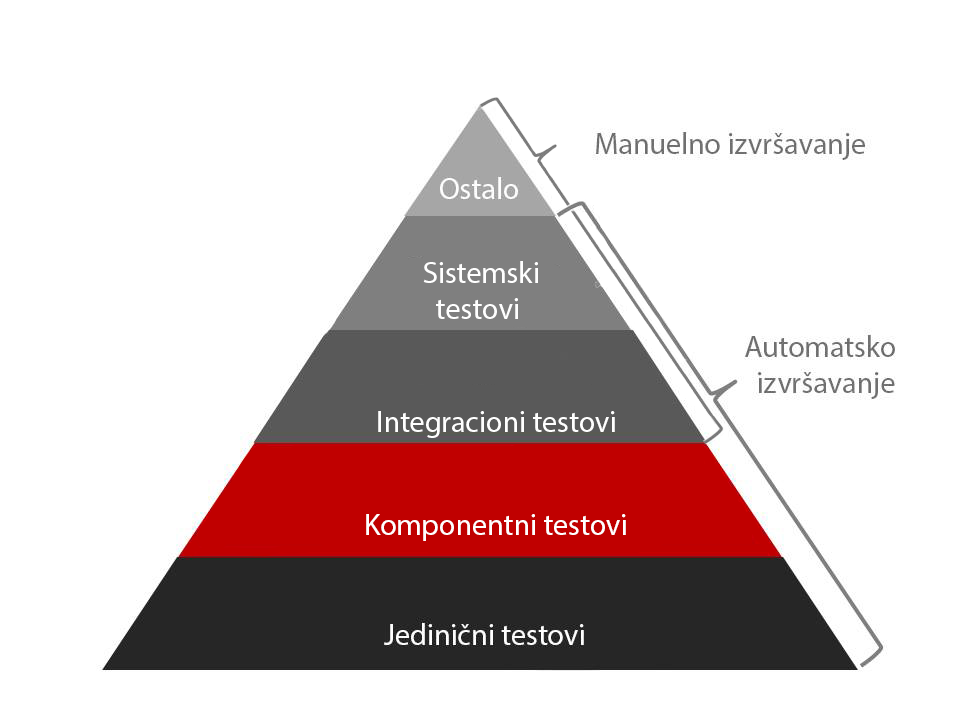
\includegraphics[width=0.9\textwidth]{piramida.png}
  \caption{Piramida testiranja softvera}
  \label{fig:piramida}
\end{figure}


Pored opisane podele i vrsta testova koji se izvršavaju, postoje i druge podele prema različitim kriterijumima testiranja. Više o podelama i podržanim načinima testiranja može se naći u literaturi \cite{TestingProcess}.

\section{Strategije testiranja} \label{broj3}
Testiranjem se obezbeđuje bolje razumevanje specifikacije problema, dizajna i implementacije rešenja. Pored otkrivanja grešaka, glavni ciljevi su obezbeđivanje traženog kvaliteta rešenja sistematskim testiranjem u kontrolisanim uslovima i identifikovanje potpunosti i korektnosti softvera. Tri najvažnije strategije za postizanje kvaliteta i detekciju grešaka su 
strategija crne kutije, strategija bele kutije i strategija sive kutije \cite{Strategies}.
 
\subsection{Strategija crne kutije}
Testiranje crnom kutijom (eng. \textit{Black Box Testing}) je strategija koja posmatra program kao zatvoreni sistem kako bi se uvrdilo ponašanje programa na
osnovu odgovarajućih ulaznih podataka \cite{BlackBoxTesting}. Ova strategija ne zahteva poznavanje strukture i analizu izvornog
koda, već samo osobine definisane specifikacijom softverskog sistema. Sprovodi se tako što se sistemu prosleđuju odgovarajući ulazni podaci a zatim se proverava da li je izlaz u skladu sa očekivanim. 
Ova strategija se između ostalog primenjuje prilikom testiranja veb aplikacija ili servisa, gde se razmatra strana koju je generisao server na osnovu unetih podataka. Strategija testiranja crne kutije obično nije najbolji pristup, ali je uvek opcija. Prednost primene ove strategije je jednostavnost, pošto testiranje može biti vođeno bez poznavanja unutrašnje
strukture softverskog sistema. Ulazni podaci za testiranje sistema definišu se tako
da povećaju verovatnoću nalaženja greške i da smanje veličinu skupa testova. Ova strategija je potpuno fokusirana na funkcionalnosti rada aplikacije. \par
U nastavku će biti opisane dve metode koje primenjuju strategiju crne kutije. To su metoda klasa ekvivalencije i metoda graničnih vrednosti.
\par 
\subsubsection{Metoda klasa ekvivalencije}
Ideja metode deljenja na klase ekvivalencije (eng. \textit{Equivalence Partitioning}) je formiranje podskupova (klasa) podataka na osnovu ulaznih podataka \cite{PartitioningBoundary}. Jedna klasa sadrži ulazne podatke koji proizvode slične rezultate (izlazne vrednosti) pri testiranju. Na primer, jednu klasu podataka mogu činiti ulazni podaci koji otkrivaju istu grešku. U idealnom slučaju, podskupovi su međusobno disjunktni i ceo ulazni skup je pokriven. 
\par 
Da bismo identifikovali klase, posmatramo specifikaciju klijentskih uslova.
Za svaki uslov kreiramo po dve klase u zavisnosti da li je uslov ispunjen ili nije. Formiramo legalne klase koje obuhvataju ispravne i očekivane ulazne podatke kao i nelegalne klase koje obuhvataja sve ostale slučajeve ulaznih podataka.
\par 
Prednost metode deljenja na klase ekvivalencije je manji utrošak vremena pri testiranju softvera usled manjeg broja proverenih test slučajeva. Ulazne vrednosti u okviru jedne klase se smatraju ekvivalentnim, pa je za svaku klasu dovoljno pokretanje samo jednog test slučaja. Proveravanjem većeg broja test slučajeva u istoj klasi, ne identifikuju se nove greške u programu.

\subsubsection{Metoda graničnih vrednosti}
Kod metode graničnih  vrednosti (eng. \textit{Boundary Value  Analysis}) test slučajevi su
napravljeni  tako  da  reprezentuju  granice  odgovarajućih 
klasa (ulaznih podataka) . Osnovu čini princip prethodno objašnjene 
metode klasa ekvivalencija \cite{PartitioningBoundary}.
Za svaki skup ulaznih podataka formiraju se tri klase, jedna validna i dve nevalidne. Validna klasa ima ispravne ulazne vrednosti, a nevalidne klase sadrže ulazne vrednosti koje ne pripadaju ispravnim opsezima. Vrednosti na granicama između validne i nevalidnih klasa nazivaju se test vektorima klasa.
Razlog  za korišćenje upravo ovih vrednosti za test vektore jesu česte softverske greške baš na
granicama opsega važenja. 

Za primenu ove metode, potrebno je više vremena za određivanje test slučajeva u poređenju sa drugim metodama strategije crne kutije zbog određivanja granica između validne i nevalidnih klasa.

\subsection{Strategija bele kutije}
Testiranje strategijom bele kutije (eng. \textit{White Box Testing}) zahteva pristup izvornom kodu, dobro poznavanje programskog jezika u kojem je sistem implementiran kao i dizajn konkrentog softverskog proizvoda \cite{WhiteBoxTesting}. Plan testiranja izvodi se proučavanjem celokupnog programskog koda. Za svaku liniju koda može se proveriti da li se ona izvršava u zavisnosti od podataka na ulazu. Takođe, može se vršiti provera izvršavanja pojedinačnih funkcija. Specifičnim testovima proverava se postojanje beskonačnih petlji ili detektovanje delova koda koji se nikad ne izvrši. 
\par
Da bi se obezbedila primena strategije bele kutije, neophodno je i poznavanje interne logike i strukture koda kako bi se dizajnirali test slučajevi koji proveravaju kontrolne strukture programskog jezika. Kontrolne strukture obuhvataju naredbe grananja, uslovne naredbe, način menjanja tokova podataka i petlje.

Metode testiranja belom kutijom su testiranje grananja, testiranje osnovnih putanja, testiranje toka podataka i testiranje petlji.
Kod testiranja grananja testira se svaka moguća odluka u kontroli toka izvršavanja. Ova metoda uključuje i testiranje u slučaju spajanje odluka.  
Testiranje osnovnih putanja prati izvršavanje blokova naredbi i u zavisnosti od izvršenih blokova formira test slučajeve za koje je potrebno pokrenuti softver. Kod testiranja toka podataka, formira se graf kontrole podataka koji sadrži informacije o pojavljivanju promenljivih u kodu i načinu njihovog menjanja. Kod testiranja petlji, proverava se ispravnost konstrukcija samih petlji.

Testiranje belom kutijom se primenjuje kod testova jedinica koda i sistemskih testova kako bi se eventualno pronašli delovi sistema koji proizvode neodgovarajuće ponašanje.
Nedostatak strategije bele kutije je visoka cena testiranja kao i zahtev za kvalifikovanim testerom. Pored toga,
mnoge putanje u sistemu mogu ostati netestirane pa se na taj način mogu sakriti potencijalne greške. 

\subsection{Strategija sive kutije}

Strategija testiranja sivom kutijom (eng. \textit{Gray Box Testing}) predstavlja kombinaciju prethodne dve strategije. Kod ove strategije postoji pristup nekom segmentu softvera, ali ne i kompletnom softverskom sistemu \cite{GrayBoxTesting}. Na osnovu analize poznatih delova koda koja odgovara testiranju bele kutije, formiraju se test slučajevi koji se zatim primenjuju na delove sistema o čijoj internoj strukturi nemamo informacija (odgovara testiranju crne kutije). Tehnika sive kutije koristi se u slučajevima testiranja integracije različitih delova koda. Ova strategija povećava pokrivenost koda test primerima kombinovanjem dve strategije. 
\par
Kada se primenjuje testiranje sivom kutijom, razlikujemo dve vrste testera. Prvu grupu čine kvalifikovani testeri koji na osnovu delimičnog pristupa izvornom kodu formiraju test slučajeve. Drugu grupu čine testeri čiji je zadatak samo izvršavanje dobijenih test slučajeva bez poznavanja interne strukture sistema. 
U zavisnosti od procenta celokupnog izvornog koda kome se može pristupiti, pokrivenost koda testovima može biti ograničena. 
\par
Metode testiranja sive kutije su ortogonalno testiranje, regresiono testiranje i testiranje obrazaca.
Ortogonalno testiranje koristi podskup svih kombinacija test slučajeva  dobijenih analizom dostupnih delova izvornog koda.
Regresioni testovi opisani su u delu \ref{broj2}. Testiranje obrazaca podrazumeva primenu testova obrazaca pri dizajnu softverskih sistema.
Ukoliko se sistem implementira prema nekom obrazcu projektovanja, testovima obrazaca proverava se da li je arhitektura sistema u skladu arhitekturom izabranog obrasca.

\section{Načini izvršavanja testova} \label{broj4}
U opštem slučaju, test se smatra uspešnim ukoliko je ponašanje sistema pri njegovom izvršavanju u skladu sa korisničkim zahtevima. Međutim, kod sve popularnije metodologije destruktivnog testiranja, test se smatra uspešnim ako se njegovim izvršavanjem otkriva postojanje greške u softveru.
\par
Izvršavanje testova sprovodi se na dva načina, automatizovano i manuelno \cite{AutomatedManualExecution}. Manuelno  testiranje predstavlja ručno izvršavanje test slučajeva izabranim alatima. 
U većini slučajeva, tester prati niz koraka da bi verifikao neki segment softverskog sistema. Nakon toga, formira se izveštaj dobijenih rezultata.
\par
Automatizovano testiranje podrazumeva postojanje određenog koda napisanog kako bi se automatizovali koraci pri izvršavanju test slučaja. 
Datoteke koje sadrže logiku za testiranje nazivaju se test skripte i mogu biti pisane u svim programskim jezicima. \par
Tokom manuelnog i automatizovanog izvršavanja testova prate se iste faze procesa testiranja koje se mogu primeniti na različite nivoe i tipove testiranja. Manuelno i automatsko izvršavanje testova ima svoje prednosti i mane. U nastavku će biti navedene neke od njih. 

Prilikom testiranja, obično su na raspolaganju ograničeni resursi, čime se onemogućuje efikasno izvršavanje manuelnih testova. Automatizovano testiranje je brže i pouzdanije jer su kod manuelnog testiranja mogući propusti usled prekomernog rada ili umora testera. Kako automatizovano izvršavanje ne zahteva prisustvo testera, oni se mogu neprekidno izvršavati.
Sa druge strane, automatizovano testiranje je skuplje i zahteva posebno kvalifikovane testere. Ušteda vremena je jako važna za velike sisteme nad kojima se između ostalog izvršavaju i regresioni testovi. Kada se sistem proširuje novom komponentom, pored već izvršenih testova, dodaju se testovi koji proveravaju funkcionalnost nove komponente. Odavde zaključujemo da je automatizacija regresionih testova neophodna zbog uštede vremena.

\par
Izvršavanje jediničnih testova i testova komponenti je uvek automatizovano. Integracioni i sistemski testovi se mogu izvršavati i automatizovano i manuelno. Istraživački i testovi prihvatljivosti se uvek izvršavaju manuelno. Načini izvršavanja testova u okviru piramide testiranja ilustrovani su slikom \ref{fig:piramida}.


\section{Načini generisanja testova} \label{broj5}

Izvršavanje testova u modernim razvojnim okruženjima je uglavnom automatizovano, ali je generisanje test slučajeva i dalje većinom manuelno. Pod manuelnim generisanjem testova podrazumevamo da tester ručno piše testove za koje će softver biti pokrenut. Ovakav način generisanja test primera može zahtevati veliki napor s obzirom da postoji veliki broj slučajeva koje je potrebno pokriti. Iz tog razloga teži se automatizaciji procesa generisanja test primera. Kod automatskog generisanja testova se korišćenjem drugih alata dobijaju test primeri za koje se pokreće softver i proverava njegovo ponašanje \cite{AutomatedTestGeneration}. \par
Jedna od tehnika automatskog generisanja test primera svodi se na formiranje testova koji pronalaze potencijalne slabosti jezika u kojem je sistem implementiran.
Na primer, za programske jezike C i C++ slabosti su prekoračenje bafera, neispravno oslobađanje memorije, dvostruko oslobađanje memorije, deljenje nulom kao i prekoračenje i potkoračenje u aritmetičkim izrazima.


\subsection{Primeri automatskog generisanja testova}
Automatizacija procesa generisanja test primera posebno je važna jer ubrzava proces testiranja. U nastavku će biti navedene neke od tehnika i alata koje imaju za cilj automatsko generisanje test primera. 


Rasplinuto testiranje (eng. \textit{Fuzz testing}) je primer tehnike koju je moguće potpuno automatizovati i zasniva se na primeni strategije crne kutije \cite{FuzzTestingForDummies}. Ovom tehnikom se generišu neispravni i neočekivani ulazi za koje se prati tok izvršavanja programa sa ciljem detektovanja nebezbednog ponašanja. Test primer sa kojim se započinje testiranje može biti slučajno generisan ili ulaz definisan od strane programera. Svaki naredni test primer generiše se na osnovu prethodno generisanih test primera, praćenja toka izvršavanja programa i promena vrednosti promenljivih. Rasplinuto testiranje može se fokusirati na granične vrednosti ulaza ali i na bilo koje ulazne vrednosti koje mogu izazvati nedefinisano ili nebezbedno ponašanje. Može se definisati i kao metod otkrivanja grešaka softvera kreiranjem neočekivanih ulaza i upravljanjem izuzecima. Danas se rasplinuto testiranje najviše koristi u velikim sistemima jer se pokazalo da ova metoda daje jako dobar odnos cene i vremena naspram kvaliteta testiranja. 
\par

Uopšteno, postoje dve vrste alata za generisanje testova primenom tehnike rasplinutog testiranja. Jedna grupa alata zahteva posebno kvalifikovane testera koji unose detalje o implementaciji sistema. Druga grupa alata omogućava generisanje testova samo konfigurisanjem parametara o očekivanom ulazu i definisanjem programskog jezika. Prednost ovog pristupa je jednostavnost, dok je mana niži kvalitet testiranja u odnosu na testove koji se formiraju za specifični sistem. 
\par
Pored navedenih osobina, postoji veliki broj metoda rasplinutog testiranja. Jedna od njih je random metoda koja je najmanje efikasna i podrazumeva generisanje slučajnog test slučaja. Zanimljiva činjenica je da su slabosti kritičnih delova softvera identifikovane upravo ovo metodom. Pored ove metode, koristi se i metoda izučavanja ulaznih vrednosti koja analizira sve podržane strukture podataka i opsege ulaznih vrednosti. Takođe, primenjuje se i rasplinuto testiranje grubom silom u kojem testiranje počinje ispravnim ulazom, a zatim se u svakom sledećem koraku menja svaki bajt ili karakter niske u zavisnosti od tipa ulazne vrednosti. Složeniji ulazi zahtevaju ogroman broj varijacija pa u tom slučaju ne postoji dobra pokrivenost testovima.
\par
Jedan od alata koji primenjuje strategiju sive kutije za automatsko generisanje test primera je SAGE \cite{ToolSAGE}. Namena alata SAGE (eng. \textit{Scalable, Automated, Guided Execution}) je proveravanje stabilnosti rada programa koji se izvršavaju na Windows operativnom sistemu čiji su procesori kompatibilni sa x86 skupom instrukcija. Odlikuje se specifičnom arhitekturom i algoritmom koji ga izdvaja od programa slične namene. Za generisanje test primera, alat SAGE koristi program koji se testira i skupove ulaznih podataka koji se jedan za drugim učitavaju u sam program. Cilj je naći skupove ulaznih podataka koji dovode do nedefinisanog i nebezbednog ponašanja tokom izvršavanja programa. Ukoliko SAGE uspe da generiše takav skup ulaznih podataka, smatra se da je on uspešno ispunio svoj zadatak. Nađeni skup podataka se zapisuje u internu bazu alata i nastavlja se potraga za drugim skupovima ulaznih podataka koji izazivaju nebezbedno ponašanje programa, ukoliko takvi postoje. Ulazni podaci se inicijalno biraju praćenjem izvršavanja programa na nivou x86 mašinskog koda. Glavni cilj alata je pokrivenost svih delova programa prolaskom kroz sve grane programa. Važno je napomenuti da se primenom ovog alata ne generišu svi mogući ulazi, s obzirom da njihovo generisanje nije moguće u razumnom roku. 
\par
Program SAGE sastoji se od četiri faze koje se izvršavaju jedna za drugom. Te faze su testiranje, praćenje mašinskih instrukcija, generisanje ograničenja i generisanje narednog skupa ulaznih podataka. Izvršavanje četiri faze predstavlja jedan ciklus. Broj ciklusa je jako veliki a ukupno izvršavanje SAGE programa meri se satima ili čak danima. 
U prvoj fazi program se izvršava koristeći početni skup ulaznih podataka. Ukoliko se tokom ove faze detektuje skup ulaznih podataka koji dovodi do nedefinisanog ponašanja programa, pronađeni skup podataka se dokumentuje u internu bazu alata. Ukoliko ovakav skup ulaznih podataka ne postoji, prelazi se na drugu fazu tokom koje formira se zapis mašinskih instrukcija na osnovu izvornog koda. Za generisanje ograničenja, koriste se blokovi mašinskih instrukcija iz prethodne faze. U poslednjoj fazi se za generisanje novih skupova ulaznih podataka koriste dobijena ograničenja a zatim sledi ponavljanje ciklusa. 
\par
KLEE \cite{ToolKLEE} je alat za simboličko izvršavanje \cite{SymbolicExecution} koji primenjuje strategiju bele kutije za automatsko generisanje test primera. 
Nastao je na univerzitetu Ilinois i javno je dostupan.
Alat proverava greške u radu sa pokazivačima, greške prekoračenja bafera i greške deljenja nulom za programe napisane u programskom jeziku C. Ovim alatom postiže se velika pokrivenost kompleksnih programa testovima. KLEE koristi razne optimizacije i heuristike za poboljšanje pokrivenosti koda prilikom simboličkog izvršavanja. Alat ima dva cilja, pokrivanje svake linije izvršnog koda u programu i detektovanje svake nebezbedne operacije ukoliko takva postoji. \par
Kod normalnog izvršavanja programa, operacije nad operandima proizvode konkretne vrednosti. Problem složenih programa je eksplozija stanja sistema koju je potrebno proveriti kako bi se generisali test primeri. Iz tog razloga, koristi se pristup simboličkog izvršavanja programa koji opisuje skup vrednosti koji je moguć na datoj putanji u programu. Kada KLEE detektuje grešku, vrši se rešavanje ograničenja trenutne putanje kako bi se proizveo test primer za koji je potrebno izvršiti program upotrebom kompajlera. 
\par 
KLEE koristi jednostavan pristup za sinhronizaciju sa okruženjem. Naime, veliki deo koda je kontrolisan vrednostima koje se dobijaju iz okruženja kao što su argumenti komandne linije i fajl sistem. 
 
\chapter{Rešavač Z3} \label{resavac}
\label{chp:razrada}

Sistemi za analizu i proveru ispravnosti softvera su veoma kompleksni. Njihovu osnovu predstavlja komponenta koja koristi logičke formule za opisivanja stanja i transformacija između stanja sistema. Opisivanje stanja sistema često se svodi na proveravanje zadovoljivosti formula logike prvog reda. 
Proveravanje zadovoljivosti formula vrši se procedurama odlučivanja u odnosu na definisanu teoriju. Formalno, zadovoljivost u odnosu na teoriju (eng. \textit{Satisfiability Modulo Theory}, skraćeno SMT) problem je odlučivanja zadovoljivosti u odnosu na osnovnu teoriju T opisanu u klasičnoj logici prvog reda sa jednakošću \cite{Barrett}. Alati koji se koriste za rešavanje ovog problema nazivaju se SMT rešavači. 
\par

Jedan od najpoznatijih SMT rešavača je rešavač Z3 kompanije Microsoft koji se koristi za proveru zadovoljivosti logičkih formula u velikom broju teorija \cite{EfficientSMTSolver}. Z3 se najčešće koristi kao podrška drugim alatima, pre svega alatima za analizu i ispitivanje ispravnosti softvera. Pripada grupi SMT rešavača sa integrisanim procedurama odlučivanja.
\par
U ovoj glavi opisane su osnove rešavača Z3 u delu \ref{sec:num1}. U delu \ref{sec:num2} opisane su najvažnije teorije uključujući teoriju neinterpretiranih funkcija, teoriju linearne aritmetike, teoriju nelinearne aritmetike, teoriju bitvektora i teoriju nizova. U delu \ref{sec:num3} opisani su  podržani tipovi podataka. U delu \ref{sec:num4} opisan je format za komunikaciju sa Z3 rešavačem korišćenjem SMT-LIB standarda. Pored toga, rešavač Z3 nudi interfejse za direktnu komunikaciju sa programskim jezicima C, C++, Java i Python. U delu \ref{sec:num5} opisan je interfejs rešavača Z3 za komunikaciju sa programskim jezikom C++. Oba formata komunikacije imaju istu moć izražajnosti. Šta više, sintaksno se jako slično zapisuju. U delu sa implementacijom biće korišćen C++ interfejs za komunikaciju sa Z3 rešavačem. Važno zapažanje je da su interfejsi za programske jezike C i C++ veoma slični. Više materijala o podržanim interfejsima za programske jezike C, C++, Java i Python može se pronaći u literaturi \cite{api}.

\section{Osnove rešavača}  \label{sec:num1}
Problem zadovoljivosti (eng. \textit{Satisfiability problem}, skraćeno SAT) problem je odlučivanja da li za iskaznu formulu u konjunktivnoj normalnoj formi postoji valuacija u kojoj su sve njene 
klauze tačne \cite{Handbook}. 
Rešavači koji se koriste za rešavanje ovog problema nazivaju se SAT rešavači.   
Rešavač Z3 integriše SAT rešavač zasnovan na savremenoj DPLL proceduri i veliki broj teorija. 
Implementiran je u programskom jeziku C++. Šematski prikaz arhitekture rešavača \cite{EfficientSMTSolver} prikazan je na slici \ref{fig:arhitektura}. 
\begin{figure}[!ht]
  \centering
  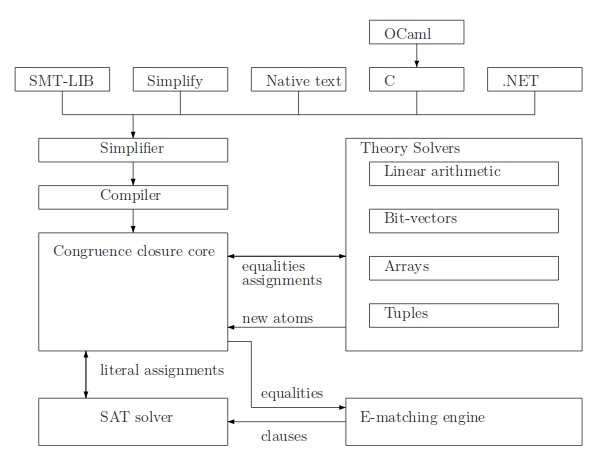
\includegraphics[width=1\textwidth]{arhitektura.png}
  \caption{Arhitektura rešavača Z3}
  \label{fig:arhitektura}
\end{figure}
\par
Formule prosleđene rešavaču se najpre procesiraju upotrebom simplifikacije. Simplifikacija primenjuje algebarska pravila redukcije kao što je \texttt{p $\land$ true $\vdash$ p}. Ovim procesom vrše se i odgovarajuće zamene kao što je \texttt{x=4 $\land$ q(x) $\vdash$ x=4 $\land$ q(4)}.
Nakon simplifikacije, kompajler formira apstraktno sintaksno stablo formula čiji su čvorovi simplifikovane formule (klauze). Zatim se jezgru kongruentnog zatvorenja (eng. 
\textit{Congruence closure core}) prosleđuje apstraktno sintaksno stablo. Jezgro kongruentnog zatvorenja komunicira sa SAT rešavačem koji određuje istinitosnu vrednost klauza. 
\par


Glavni gradivni blokovi formula su konstante, funkcije i relacije. Konstante su specijalan slučaj funkcija bez parametara. Svaka konstanta je određene sorte. Sorta odgovara tipu u programskim jezicima. Relacije su funkcije koje vraćaju povratnu vrednost tipa Boolean. Funkcije mogu uzimati argumente tipa Boolean pa se na taj način relacije mogu koristiti kao argumenti funkcija.  


Formula $F$ je validna ako je vrednost valuacije $true$ za bilo koje interpretacije funkcija i konstantnih simbola. Formula $F$ je zadovoljiva ukoliko postoji bar jedna valuacija u kojoj je formula tačna. Da bismo odredili da li je formula $F$ validna, rešavač Z3 proverava da li je formula $\lnot F$ zadovoljiva. Ukoliko je negacija formule nezadovoljiva, onda je polazna formula validna. 



\section{Teorije} \label{sec:num2}
Teorije rešavača Z3 su opisane u okviru višesortne logike prvog reda sa jednakošću.  Definisanjem specifične teorije, uvode se restrikcije pri definisanju formula kao i podržanih relacija i operatora koje se nad njima primenjuju. Na taj način, specijalizovane metode u odgovarajućoj teoriji mogu biti efikasnije implementirane u poređenju sa opštim slučajem. U nastavku će biti opisane teorija neinterpretiranih funkcija, teorija linearne aritmetike, teorija nelinearne aritmetike, teorija bitvektora i teorija nizova.

\subsection{Teorija neinterpretiranih funkcija}
Teorije obično određuju interpretaciju funkcijskih simbola. Teorija koja ne zadaje nikakva ograničenja za funkcijske simbole naziva se teorija neinterpretiranih funkcija 
(eng. \textit{Theory of Equality with Uninterpreted Functions}, skraćeno EUF). \par Kod rešavača Z3, funkcije i konstantni simboli su neinterpretirani. Ovo je kontrast u odnosu na funkcije odgovarajućih teorija. Funkcija + ima standardnu interpretaciju u teoriji aritmetike. Neinterpretirane funkcije i konstante su maksimalno fleksibilne i dozvoljavaju bilo koju interpretaciju koja je u skladu sa ograničenjima. Za razliku od programskih jezika, funkcije logike prvog reda su totalne, tj. definisane su za sve vrednosti ulaznih parametara. Na primer, deljenje 0 je dozvoljeno, ali nije specifikovano šta ono predstavlja. Teorija neinterpretiranih funkcija je odlučiva i postoji procedura odlučivanja polinomijalne vremenske složenosti. Jedna od procedura odlučivanja za ovu teoriju zasniva se na primeni algoritma Nelson-Open (eng. \textit{Nelson-Open algorithm}). O ovom algoritmu može se više naći u literaturi \cite{NelsonOpen}.
\par



\subsection{Teorija linearne aritmetike} 

Rešavač Z3 sadrži procedure odlučivanja za linearnu aritmetiku nad celobrojnim i realnim brojevima. Dodatni materijali o procedurama odlučivanja linearne aritmetike dostupni su u literaturi \cite{FastLinearArithmetic}.
\par

U okviru celobrojne linearne aritmetike, podržani funkcijski simboli su $+$, $-$ i $*$ pri čemu je kod množenja drugi operand konstanta. Nad funkcijskim simbolima, čiji su specijalni slučajevi konstante mogu se primenjivati relacijski operatori $<$, $\leq$, $>$ i $\geq$. 
\par
U okviru realne linearne aritmetike, podržani funkcijski simboli su $+$, $-$ i $*$ pri čemu je kod operacije množenja drugi operand konstanta. Pored ovih podržane su operacije $div$ i $mod$, uz uslov da je drugi operand konstanta različita od 0. Nad funkcijskim simbolima, čiji su specijalni slučajevi konstante mogu se primenjivati relacijski operatori $<$, $\leq$, $>$ i $\geq$. 
\par
\subsection{Teorija nelinearne aritmetike} 

Formula predstavlja formulu nelinearne aritmetike ako je oblika (* t s), pri čemu t i s nisu linearnog oblika.
Nelinearna celobrojna aritmetika je neodlučiva, tj. ne postoji procedura koja za proizvoljnu formulu vraća zadovoljivost ili nezadovoljivost. U najvećem broju slučajeva, Z3 vraća nepoznat rezultat. Za nelinearne probleme, rešavač Z3 koristi posebne metode odlučivanja zasnovane na Grebnerovim bazama. 


\subsection{Teorija bitvektora} 
Rešavač Z3 podržava bitvektore proizvoljne dužine. \texttt{(\_ BitVec n)} je sorta bitvektora čija je dužina \texttt{n}. Bitvektor literali se mogu definisati koristeći binarnu, decimalnu ili heksadecimalnu notaciju. U binarnom i heksadecimalnom slučaju, veličina bitvektora je određena brojem karaktera. Na primer, literal \textit{\#b010} u binarnom formatu je bitvektor dužine 3. Kako konstanta \textit{a} u heksadecimalnom formatu odgovara vrednosti 10, literal \textit{\#x0a} je bitvektor veličine 10. Veličina bitvektora mora biti specifikovana u decimalnom formatu. Na primer, reprezentacija \textit{(\_ bv10 32)} je bitvektor dužine 32 sa vrednošću 10. Podrazumevano, Z3 predstavlja bitvektore u heksadecimalnom formatu ukoliko je dužina bitvektora umnožak broja 4 a u suprotnom u binarnom formatu. Bitvektor literali mogu biti reprezentovani u decimalnom formatu. Više materijala o procedurama odlučivanja za teoriju bitvektora može se naći u literaturi \cite{DPBitvector}.

Pri korišćenju operatora nad bitvektorima, mora se eksplicitno navesti tip operatora. Zapravo, za svaki operator podržane su dve varijante za rad sa označenenim i neoznačenim operandima. Ovo je kontrast u odnosu na programske jezike u kojima kompajler na osnovu argumenata implicitno određuje tip operacije (označena ili neoznačena varijanta).
\par
U skladu sa prethodno navedenom činjenicom, teorija bitvektora ima na raspolaganju različite verzije aritmetičkih operacija za označene i neoznačene operande. Za rad sa bitvektorima od aritmetičkih operacija definisane su operacije sabiranja, oduzimanja, određivanje negacije (zapisivanja broja u komplementu invertovanjem svih bitova polaznog broja), množenja, izračunavanja modula pri deljenju, šiftovanje u levo kao i označeno i neoznačeno šiftovanje u desno. Podržane su sledeće logičke operacije: disjunkcija, konjunkcija, unarna negacija, negacija konjunkcije i negacija disjunkcije. Definisane su različite relacije nad bitvektorima kao što su $\leq$, $<$, $\geq$ i $>$.



\subsection{Teorija nizova} 
Osnovnu teoriju nizova karakterišu \texttt{select} i \texttt{store} funkcije. 
Funkcijom \texttt{(select a i)} vraća se vrednost na poziciji i u nizu a, dok se funkcijom \texttt{(store a i v)} formira novi niz, identičan nizu a pri čemu se na poziciji i nalazi vrednost v.
Z3 sadrži procedure odlučivanja za osnovnu teoriju nizova.
Dva niza su jednaka ukoliko su vrednosti svih elemenata na odgovarajućim pozicijama jednake.
 

\subsubsection{Konstantni nizovi}

Nizovi sa konstantnim vrednostima mogu se specifikovati koristeći \texttt{const} konstrukciju. Prilikom upotrebe \texttt{const} konstrukcije rešavač Z3 ne može da odluči kog tipa su elementi niza pa se on mora eksplicitno navesti. Interpretacija nizova je slična interpretaciji funkcija. Z3 koristi konstrukciju \texttt{(\_ as-array f)} za određivanje interpretacije niza. Ako je niz a jednak rezultatu konstrukcije \texttt{(\_ as-array f)}, tada za svaki indeks i, vrednost \texttt{(select a i)} odgovara vrednosti \texttt{(f i)}. 


\subsubsection{Primena map funkcije na nizove}
Rešavač Z3 obezbeđuje primenu parametrizovane funkcije \texttt{map} na nizove. Funkcijom \texttt{map} omogućava se primena proizvoljnih funkcija na sve elemente niza.

Nad nizovima se mogu vršiti slične operacije kao i nad skupovima. Rešavač Z3 ima podršku za računanje unije, preseka i razlike dva niza. Ovi operatori se tumače na isti način kao i u teoriji skupova. Za nizove a i b, pomenuti operatori mogu se koristiti navođenjem funkcija:\\
\texttt{(union a b)} ; kreiranje unije dva niza kao skupa \\
\texttt{(intersect a b)} ; kreiranje preseka dva niza kao skupa \\
\texttt{(difference a b)} ; kreiranje razlike dva niza kao skupa

\section{Tipovi podataka} \label{sec:num3}
U okviru rešavača Z3 dostupni su primitivni tipovi podataka, definisanjem konstanti različitih sorti. Neke od najčešće korišćenih su konstante bulovske, celobrojne i realne sorte.
Pored toga, mogu se definisati algebarski tipovi podataka. Algebarski tipovi podataka omogućavaju specifikaciju uobičajnih struktura podataka. Slogovi, torke i skalari (enumeracijski tipovi) spadaju u algebarske tipove podataka. Primena algebarskih tipova podataka može se generalizovati. Mogu se koristiti za specifikovanje konačnih listi, stabala i rekurzivnih struktura. 
\subsubsection{Slogovi}
Slog se specifikuje kao tip podataka sa jednim konstruktorom i proizvoljnim brojem elemenata sloga. Rešavač Z3 ne dozvoljava povećavanje broja argumenata sloga nakon njegovog definisanja. Važi svojstvo da su dva sloga jednaka samo ako su im svi argumenti jednaki.
\subsubsection{Skalari (tipovi enumeracije)}

Sorta skalara je sorta konačnog domena. Elementi konačnog domena se tretiraju kao različite konstante. Na primer, neka je S skalarni tip sa tri vrednosti A, B i C. Moguće je da tri konstante skalarnog tipa S budu različite. Ovo svojstvo ne može važiti u slučaju četiri konstante.


\subsubsection{Rekurzivni tipovi podataka}

Deklaracija rekurzivnog tipa podataka uključuje sebe direktno kao komponentu. Standardni primer rekurzivnog tipa podataka je lista. 
Lista celobrojnih vrednosti sa imenom \texttt{list} može se deklarisati naredbom:\\
\texttt{(declare-datatypes (list (nil) ((head Int) (tail list)))}
\par
Rešavaš Z3 ima ugrađenu podršku za liste korišćenjem ključne reči \texttt{List}.
Prazna lista se definiše korišćenjem klučne reči \texttt{nil} a konstruktor \texttt{insert} se koristi za dodavanje elemenata u listu. Selektori \texttt{head} i \texttt{tail} se definišu na uobičajan način.


\section{Upotreba rešavača korišćenjem SMT-LIB standarda} \label{sec:num4}
Ulazni format rešavača Z3 je definisan SMT-LIB 2.0 standardom \cite{SMTLIB}. Standard definiše jezik logičkih formula čija se zadovoljivost proverava u odnosu na neku teoriju. Cilj standarda je pojednostavljivanje jezika logičkih formula povećavanjem njihove izražajnosti i fleksibilnosti kao i obezbeđivanje zajedničkog jezika za sve SMT rešavače. 
\par
Interno, Z3 održava stek korisnički definisanih formula i deklaracija. Formule i deklaracije jednim imenom nazivamo tvrđenjima. Komandom \texttt{push} kreira se novi opseg i čuva se trenutna veličina steka. Komandom \texttt{pop} uklanjaju se sva tvrđenja i deklaracije zadate posle push-a sa kojim se komanda uparuje. Komandom \texttt{assert} dodaje se formula na interni stek. Skup formula na steku je zadovoljiv ako postoji interpretacija u kojoj sve formule imaju istinitosnu vrednost tačno. Ova provera se vrši komandom \texttt{check-sat}. U slučaju zadovoljivosti vraća se \texttt{sat}, u slučaju nezadovoljivosti vraća se \texttt{unsat} a kada rešavač ne može da proceni da li je formula zadovoljiva ili ne vraća se \texttt{unknown}. Komandom \texttt{get-model} vraća se interpretacija u kojoj su sve formule na steku tačne. 
\par

Komandom \texttt{declare-const} deklariše se konstanta odgovarajuće sorte. Sorta može biti parametrizovana i u tom slučaju su specifikovana imena njenih parametara. Naredbom \texttt{(define-sort [symbol] ([symbol]+)[sort])} vrši se specifikacija sorte.
Komandom \texttt{declare-fun} deklariše se funkcija. 
U primeru \ref{example1} koristimo činjenicu da se validnost formule pokazuje ispitivanjem zadovoljivosti negirane formule. 

\begin{primer} \label{example1} Dokazivanje de Morganovog zakona dualnosti\label{primer:demorgan} ispitivanjem validnosti formule: $\neg{(a \land b)} \Leftrightarrow (\neg{a} \lor \neg{b}) $ tako što se kao ograničenje dodaje negacija polazne formule. Z3 pronalazi da je negacija formule nezadovoljiva, pa je polazna formula tačna u svim interpretacijama. \\

\hspace{-0.6cm}
\begin{minipage}[b]{0.5\textwidth}
\textbf{Formula prosleđena rešavaču:}
\\(declare-const a Bool)
\\(declare-const b Bool)
\\(define-fun demorgan () Bool
\\\tab (= (and a b) (not (or (not a) (not b))))
\\)
\\(assert (not demorgan))
\\(check-sat) 
\\(get-model)
\end{minipage}
\hspace{1.5cm}
\begin{minipage}[t]{0.4\textwidth}
\vspace{-5.35cm}
\textbf{Izlaz:}
\\unsat
\end{minipage}
\end{primer}

Rešavač Z3 ima podršku za celobrojne i realne konstante. Komandom \texttt{declare-const} deklarišu se celobrojne i realne konstante. Rešavač ne vrši automatsku konverziju između celobrojnih i realnih konstanti. Ukoliko je potrebno izvršiti ovakvu konverziju koristi se funkcija \texttt{to-real} za konvertovanje celobrojnih u realne vrednosti.
Realne konstante treba da budu zapisane sa decimalnom tačkom. Primer \ref{example2} ilustruje deklarisanje konstanti i funkcija kao i primenu funkcije na konstante. Ispituje se zadovoljivost ograničenja.

\begin{primer} \label{example2} 
Rešavaču se prosleđuje ograničenja koje sadrže primenu funkcije f na celobrojnu konstantu a kao i relacijske operatore. Rešavač Z3 pronalazi da je ovo tvrđenje zadovoljivo i daje prikazani model. 
\\ 

\hspace{-0.7cm}
\begin{minipage}[b]{0.43\textwidth}
\textbf{Formula prosleđena rešavaču:}\\
(declare-const a Int)\\
(declare-fun f (Int Bool) Int)\\
(assert (> a 10))\\
(assert (< (f a true) 100))\\
(check-sat)\\
(get-model) \\
\end{minipage}
\hspace{0.6cm}
\begin{minipage}[t]{0.5\textwidth}
\vspace{-4.715cm}
\textbf{Izlaz:}
\\sat 
\\(model 
\\\tab(define-fun a () Int 11) 
\\\tab(define-fun f ((x!1 Int) (x!2 Bool)) Int 
\\\tab(ite (and (= x!1 11) (= x!2 true)) 0 0))
\\)
\end{minipage}
\end{primer}

Primer \ref{example3} ilustruje pronalaženje interpretacija celobrojnih i realnih konstanti. Interpretacija se svodi na pridruživanje brojeva svakoj konstanti. 

\begin{primer} \label{example3} 
Rešavaču se prosleđuju jednostavna ograničenja za celobrojne i realne konstante.
Ograničenja sadrže aritmetičke i relacijske operatore. Rešavač vraća zadovoljivost tvrđenja i dobijeni model prikazujemo u nastavku.\\ \\
\begin{minipage}[b]{0.47\textwidth}
\textbf{Formula prosleđena rešavaču:}
\\(declare-const a Int)
\\(declare-const b Int)
\\(declare-const c Int)
\\(declare-const d Real)
\\(declare-const e Real)
\\(assert (> e (+ (to\_real (+ a b)) 2.0)))
\\(assert (= d (+ (to\_real c) 0.5)))
\\(check-sat)
\\(get-model)
\end{minipage}
\hspace{1.6cm}
\begin{minipage}[t]{0.4\textwidth}
\vspace{-6cm}
\textbf{Izlaz:}
\\sat 
\\(model
\\\tab(define-fun b () Int 0) 
\\\tab(define-fun a () Int 1) 
\\\tab(define-fun e () Real 4.0) 
\\\tab(define-fun c () Int 0) 
\\\tab(define-fun d () Real (/ 1.0 
\\\tab 2.0))
\\)
\end{minipage}

\end{primer}


Takođe, postoji uslovni operator (if-then-else operator). Na primer,
izraz (ite (and (= x!1 11) (= x!2 false)) 21 0) ima vrednost 21 kada je promenljiva x!1 jednaka 11, a promenljiva x!2 ima vrednost False. U suprotnom, vraća se 0.

U slučaju deljenja, može se koristiti \texttt{ite} (if-then-else) operator i na taj način se može dodeliti interpretacija u slučaju deljenja nulom.
\par
Mogu se konstruisati novi operatori, korišćenjem \texttt{define-fun} konstruktora. Ovo je zapravo makro, pa će rešavač vršiti odgovarajuće zamene. U primeru \ref{example4} ilustruje se definisanje novog operatora. Zatim se novi operator primenjuje na konstante, uvode se ograničenja i ispituje njihova zadovoljivost.
\begin{primer} \label{example4}
Definišemo operator deljenja tako da rezultat bude specifikovan i kada je delilac 0. Uvode se dve konstante realnog tipa i primenjuje se definisani operator. Z3 rešavač pronalazi nezadovoljivost tvrđenja s obzirom da operator \texttt{mydiv} vraća 0 pa relacija poređenja ne može biti tačna.\\ \\
\begin{minipage}[b]{0.5\textwidth}
\textbf{Formula prosleđena rešavaču:}
\\(define-fun mydiv ((x Real) (y Real)) Real
\\\tab (if (not (= y 0.0))  (/ x y)  0.0))
\\(declare-const a Real)
\\(declare-const b Real)
\\(assert (>= (mydiv a b) 1.0))
\\(assert (= b 0.0))
\\(check-sat)
\end{minipage}
\hspace{3cm}
\begin{minipage}[t]{0.4\textwidth}
\vspace{-4.73cm}
\textbf{Izlaz:}
\\unsat
\end{minipage}
\end{primer}
\par
Primer \ref{example5} ilustruje rešavanje nelinearnog problema uvođenjem ograničenja nad realnim konstantama. Ispituje se zadovoljivost prosleđenih ograničenja. Kada su prisutna samo nelinearna ograničenja nad realnim konstantama, Z3 koristi posebne metode odlučivanja\begin{primer} \label{example5} Rešavaču se prosleđuje ograničenja $b^{3} + b*c = 3$ nad realnim konstantama. Rešavač vraća zadovoljivost tvrđenja i dobijeni model prikazujemo u nastavku.   
\\ \\
\begin{minipage}[b]{0.43\textwidth}
\textbf{Formula prosleđena rešavaču:}
\\(declare-const b Real)
\\(declare-const c Real)
\\(assert (= (+ (* b b b) (* b c)) 3.0))
\\(check-sat)
\\(get-model)

\end{minipage}
\hspace{1.5cm}
\begin{minipage}[t]{0.45\textwidth}
\vspace{-3.4cm}
\textbf{Izlaz:}
\\sat 
\\(model 
\\\tab(define-fun b () Real (/ 1.0 8.0)) 
\\\tab(define-fun c () Real (/ 15.0 64.0))
\\)
\end{minipage}
\end{primer}
\par
Primer \ref{example6} ilustruje različite načine predstavljanja bitvektora. Ukoliko zapis počinje sa \#b, bitvektor se zapisuje u binarnom formatu. Ukoliko zapis počinje sa \#x, bitvektor se zapisuje u heksadecimalnom formatu.
\begin{primer} \label{example6} 
Nakon specifikacije formata, zapisuje se dužina vektora. Drugi način zapisa počinje skraćenicom \texttt{bv}, navođenjem vrednosti i na kraju dužine. Komandom \texttt{(display t)} štampa se izraz \texttt{t}.\\\\
\begin{minipage}[b]{0.45\textwidth}
\textbf{Formula prosleđena rešavaču:}
\\(display \#b0100)
\\(display (\_ bv20 8))
\\(display (\_ bv20 7))
\\(display \#x0a) 
\\(set-option :pp.bv-literals false)
\\(display \#b0100)
\\(display (\_ bv20 8))
\\(display (\_ bv20 7))
\\(display \#x0a)
\end{minipage}
\hspace{2.5cm}
\begin{minipage}[t]{0.4\textwidth}
\vspace{-5.93cm}
\textbf{Izlaz:}
\\\#x4 
\\\#x14 
\\\#b0010100 
\\\#x0a 
\\(\_ bv4 4) 
\\(\_ bv20 8) 
\\(\_ bv20 7) 
\\(\_ bv10 8)
\end{minipage}
\end{primer}
\par Primer \ref{example7} ilustruje primenu aritmetičkih operacija nad bitvektorima. Podržane aritmetičke operacije su sabiranje \texttt{(bvadd)}, oduzimanje \texttt{(bvsub)}, unarna negacija \texttt{(bvneg)}, množenje \texttt{(bvmul)}, računanje modula \texttt{(bvmod)}, šiftovanje ulevo \texttt{(bvshl)}, neoznačeno (logičko) šiftovanje udesno \texttt{(bvlshr)} i označeno (aritmetičko) šiftovanje udesno \texttt{(bvashr)}. Od logičkih operacija postoji podrška za disjunkciju \texttt{(bvor)}, konjunkciju \texttt{(bvand)}, ekskluzivnu disjunkciju \texttt{(bvxor)}, negaciju disjunkcije \texttt{(bvnor)}, negaciju konjunkcije \texttt{(bvnand)} i negaciju ekskluzivne disjunkcije \texttt{(bvnxor)}.
\begin{primer} \label{example7} 
Ovaj primer ilustruje primenu nekih aritmetičkih operacija nad bitvektorima i dobijene rezultate. Komandom \texttt{(simplify t)} prikazuje se jednostavniji izraz ekvivalentan izrazu \texttt{t} ukoliko postoji.
\\ \\
\begin{minipage}[b]{0.5\textwidth}
\textbf{Formula prosleđena rešavaču:}
\\(simplify (bvadd \#x07 \#x03)) 
\\(simplify (bvsub \#x07 \#x03)) 
\\(simplify (bvneg \#x07))       
\\(simplify (bvmul \#x07 \#x03)) 
\\(simplify (bvsmod \#x07 \#x03)) 
\\(simplify (bvshl \#x07 \#x03)) 
\\(simplify (bvlshr \#xf0 \#x03))  
\\(simplify (bvashr \#xf0 \#x03))  
\\(simplify (bvor \#x6 \#x3)) 
\\(simplify (bvand \#x6 \#x3))   
\end{minipage}
\hspace{2.5cm}
\begin{minipage}[b]{0.5\textwidth}
\textbf{Izlaz:}
\\\#x0a 
\\\#x04 
\\\#xf9 
\\\#x15 
\\\#x01 
\\\#x38 
\\\#x1e 
\\\#xfe
\\\#x7 
\\\#x2 
\end{minipage}

\end{primer} \par
Postoji brz način da se proveri da li su brojevi fiksne dužine stepeni dvojke. U primeru \ref{example8} pokazuje se da je bitvektor x stepen dvojke ako i samo ako je vrednost izraza x $\land$ (x - 1) jednaka 0.

\begin{primer} \label{example8}
Provera da li je broj stepen dvojke primenjuje se na bitvektore čije su vrednosti 0, 1, 2, 4 i 8. Rešavaču se prosleđuje negacija formule. U svim slučajevima brojevi su stepeni dvojke pa Z3 rešavač vraća nezadovoljivost.\\ \\
\begin{minipage}[b]{0.5\textwidth}
\textbf{Formula prosleđena rešavaču:}
\\(define-fun is-power-of-two 
\\\tab((x (\_ BitVec 4))) Bool 
\\\tab(= \#x0 (bvand x (bvsub x \#x1)))
\\)
\\(declare-const a (\_ BitVec 4))
\\(assert 
\\\tab(not (= (is-power-of-two a) 
\\\tab\tab    (or (= a \#x0) 
\\\tab\tab\tab     (= a \#x1) 
\\\tab\tab\tab     (= a \#x2) 
\\\tab\tab\tab     (= a \#x4) 
\\\tab\tab\tab     (= a \#x8)
\\\tab\tab		))
\\\tab )
\\)
\\(check-sat)
\end{minipage}
\hspace{2.5cm}
\begin{minipage}[t]{0.5\textwidth}
\vspace{-10.45cm}
\textbf{Izlaz:}
\\unsat
\end{minipage}
\end{primer}
\par Primer \ref{example9} ilustruje upotrebu relacija nad bitvektorima. Podržane relacije uključuju neoznačene i označene verzije za operatore $<$, $\leq$, $>$ i $\geq$. Neoznačene varijante počinju nazivom \texttt{bvu}, a u nastavku sledi ime relacije. Označene varijante počinju nazivom \texttt{bvs}, a u nastavku ponovo sledi ime relacije. 
\begin{primer} \label{example9} Primer ilustruje upotrebu označenih i neoznačenih verzija operatora nad bitvektorima. Na primer, relacija $\leq$ nad neoznačenim brojevima zadaje se komandom \texttt{bvule}, a relacija $>$ nad neoznačenim brojevima komandom \texttt{bvugt}. Slično, relacija $\geq$ nad neoznačenim brojevima zadaje se komandom \texttt{bvsge}, a relacija $<$ nad označenim brojevima komandom \texttt{bvslt}.
\\ \\ 
\begin{minipage}[b]{0.5\textwidth}
\textbf{Formula prosleđena rešavaču:}
\\(simplify (bvule \#x0a \#xf0))  
\\(simplify (bvult \#x0a \#xf0))  
\\(simplify (bvuge \#x0a \#xf0))  
\\(simplify (bvugt \#x0a \#xf0))  
\\(simplify (bvsle \#x0a \#xf0)) 
\\(simplify (bvslt \#x0a \#xf0))  
\\(simplify (bvsge \#x0a \#xf0))  
\\(simplify (bvsgt \#x0a \#xf0))

\end{minipage}
\hspace{2cm} 
\begin{minipage}[t]{0.5\textwidth}
\vspace{-5.3cm}
\textbf{Izlaz:}
\\true 
\\true 
\\false 
\\false 
\\false 
\\false 
\\true 
\\true
\end{minipage}


\end{primer}

Rešavač Z3 nudi funkcije za promenu načina reprezentacije brojeva. Moguće su konverzije reprezentacije brojeva linearne aritmetike u reprezentaciju bitvektora i obrnuto. Ovaj rezultat može se postići naredbama: \\
\texttt{(define b (int2bv[32] z))} \\  
\texttt{(define c (bv2int[Int] x))}
\par
Primer \ref{example10} ilustruje poređenje bitvektora koristeći označene i neoznačene verzije operatora. Ispituje se zadovoljivost prosleđenog ograničenja.
\begin{primer} \label{example10} Označeno poređenje, kao što je bvsle, uzima u obzir znak bitvektora za poređenje, dok neoznačeno poređenje komandom bvule tretira bitvektor kao prirodan broj. Z3 rešavač pronalazi da je tvrđenje zadovoljivo i daje prikazani model.
\\ \\
\begin{minipage}[b]{0.5\textwidth}
\textbf{Formula prosleđena rešavaču:}
\\(declare-const a (\_ BitVec 4))
\\(declare-const b (\_ BitVec 4))
\\(assert (not (= (bvule a b) (bvsle a b)))
\\(check-sat)
\\(get-model)
\end{minipage}
\hspace{1.15cm} 
\begin{minipage}[t]{0.5\textwidth}
\vspace{-3.45cm}
\textbf{Izlaz:}
\\sat 
\\(model 
\\\tab(define-fun b () (\_ BitVec 4) \#xe) 
\\\tab(define-fun a () (\_ BitVec 4) \#x0)
\\)
\end{minipage}
\end{primer}
\par
Primer \ref{example11} ilustruje kako se definišu nizovi sa konstantnim vrednostima. Zatim se dodaju ograničenja korišćenjem funkcije \texttt{select} i ispituje se njihova zadovoljivost.
\begin{primer} \label{example11} Definišemo konstantni niz m celobrojnog tipa i dve celobrojne konstante a i i. Uvodimo ograničenje da niz m sadrži samo jedinice. Z3 pronalazi da je ovo tvrđenje zadovoljivo i daje prikazani model.\\
\begin{minipage}[b]{0.55\textwidth}
\vspace{0.5cm} 
\textbf{Formula prosleđena rešavaču:}
\\(declare-const m (Array Int Int))
\\(declare-const a Int)
\\(declare-const i Int)
\\(assert (= m ((as const (Array Int Int)) 1)))
\\(assert (= a (select m i)))
\\(check-sat)
\\(get-model)
\end{minipage}
\hspace{1.1cm} 
\begin{minipage}[t]{0.5\textwidth}
\vspace{-4.7cm}
\textbf{Izlaz:}
\\sat 
\\(model 
\\\tab(define-fun m () (Array Int Int) 
\\\tab\tab(\_ as-array k!0)
\\\tab) 
\\\tab(define-fun i () Int 0) 
\\\tab(define-fun a () Int 1) 
\\\tab(define-fun k!0 ((x!0 Int)) 
\\\tab\tab Int (ite (= x!0 0) 1 1)
\\\tab)
\\)
\end{minipage}
\end{primer}
\par
Primer \ref{example12} ilustruje primenu funkcije \texttt{map} na sve elemente konstatnih nizova. Za svaka dva elementa koji pripadaju različitim nizovima, pokazuje se važenje De Morganovog zakona iz primera \ref{example1}. 
\begin{primer} \label{example12} 
Kao ograničenje dodajemo negaciju navedene formule. Rešavač Z3 vraća nezadovoljivost negirane formule, odakle zaključujemo da je polazna formula validna.\\ \\
\begin{minipage}[b]{0.65\textwidth}
\textbf{Formula prosleđena rešavaču:}
\\(define-sort Set (T) (Array T Bool))
\\(declare-const a (Set Int))
\\(declare-const b (Set Int))
\\(assert (not (= ((\_ map and) a b) ((\_ map not) 
\\\tab((\_ map or) ((\_ map not) b) ((\_ map not) a)))))
\\)
\\(check-sat)
\end{minipage}
\hspace{2.5cm} 
\begin{minipage}[t]{0.5\textwidth}
\vspace{-4.65cm}
\textbf{Izlaz:}
\\unsat 
\end{minipage}
\end{primer}

\par
U primeru \ref{example13} pokazuje se da su dva sloga jednaka ako i samo ako su im svi argumenti jednaki. Uvodi se parametarski tip \texttt{Pair} i koriste se selektorske funkcije \texttt{first} i \texttt{second}. 

\begin{primer} \label{example13} Nakon definisanja slogova p1 i p2, dodaje se ograničenje koje se odnosi na drugi element sloga.
Dodajemo i ograničenje da su slogovi p1 i p2 jednaki. Rešavač Z3 vraća zadovoljivost formule i odgovarajući model. 
\\ \\
\begin{minipage}[b]{0.5\textwidth}
\textbf{Formula prosleđena rešavaču:}
\\(declare-datatypes (T1 T2) 
\\\tab[0.3cm](Pair (mk-pair (first T1) (second T2))))
\\(declare-const p1 (Pair Int Int))
\\(declare-const p2 (Pair Int Int))
\\(assert (= p1 p2))
\\(assert (> (second p1) 20))
\\(check-sat)
\\(get-model)
\end{minipage}
\hspace{1.5cm} 
\begin{minipage}[t]{0.5\textwidth}
\vspace{-5.35cm}
\textbf{Izlaz:}
\\sat 
\\(model 
\\\tab(define-fun p1 () (Pair Int Int) 
\\\tab\tab(mk-pair 0 21)
\\\tab) 
\\\tab(define-fun p2 () (Pair Int Int) 
\\\tab\tab(mk-pair 0 21)
\\\tab)
\end{minipage}

\end{primer}
\par
U primeru \ref{example14} ilustruje se definisanje listi kao i dodavanje ograničenja korišćenjem selektorskih funkcija \texttt{head} i \texttt{tail}. Ispituje se zadovoljivost tvrđenja.
\begin{primer} \label{example14}
Pored ograničenja za prve elemente listi, tražimo model takav da liste l1 i l2 nisu jednake, tj. da nisu svi elementi na odgovarajućim pozicijama u listama jednaki. Rešavač Z3 vraća zadovoljivost tvrđenja i dobijeni model prikazujemo u nastavku.
\\ \\
\begin{minipage}[b]{0.42\textwidth}
\textbf{Formula prosleđena rešavaču:}
\\(declare-const l1 (List Int))
\\(declare-const l2 (List Int))
\\(declare-const l3 (List Int))
\\(declare-const x Int)
\\(assert (not (= l1 nil)))
\\(assert (not (= l2 nil)))
\\(assert (= (head l1) (tail l2)))
\\(assert (not (= l1 l2)))
\\(assert (= l3 (insert x l2)))
\\(assert (> x 100))
\\(check-sat)
\\(get-model)
\end{minipage}
\hspace{0.9cm}
\begin{minipage}[t]{0.55\textwidth}
\vspace{-7.84cm}
\textbf{Izlaz:}
\\sat 
\\(model 
\\\tab(define-fun l3 () (List Int) 
\\\tab(insert 101 (insert 0 (insert 1 nil)))
\\\tab(define-fun x () Int 101) 
\\\tab(define-fun l1 () (List Int) (insert 0 nil)) 
\\\tab(define-fun l2 () (List Int) (insert 0 
\\\tab\tab(insert 1 nil))
\\\tab)
\\) 
\end{minipage}


\end{primer}

U prethodnom primeru, uvode se ograničenja da su liste l1 i l2 različite od \texttt{nil}. Ova ograničenja se uvode jer interpretacija selektora \texttt{head} i \texttt{tail} 
nije specifikovana u slučaju praznih lista.



\section{Upotreba rešavača korišćenjem C++ interfejsa} \label{sec:num5}
C++ interfejs prema rešavaču Z3 obezbeđuje različite strukture podataka, klase i funkcije koje su potrebne za direktnu komunikaciju C++ aplikacije sa rešavačem. Neke od najbitnijih klasa biće opisane u nastavku, dok se kompletan opis interfejsa može naći na internetu \cite{cppapi}.

Klasa \texttt{Z3\_sort} koristi se za definisanje sorte izraza.  Prilikom definisanja izraza navodi se sorta kako bi bio poznat skup vrednosti koje mu se mogu dodeliti kao i skup dozvoljenih metoda. Sorte izraza definisane su tipom enumeracije. Neke od najvažnijih sorti su \texttt{Z3\_BOOL\_SORT}, \texttt{Z3\_INT\_SORT}, \texttt{Z3\_REAL\_SORT}, \texttt{Z3\_BV\_SORT} i \texttt{Z3\_ARRAY\_SORT}. Određivanje sorte izraza vrši se funkcijom \texttt{sort\_kind()} sa povratnom vrednošću tipa enumeracije. Za proveru pripadnosti izraza sorti, koriste se funkcije \texttt{is\_bool()}, \texttt{is\_int()}, \texttt{is\_real()}, \texttt{is\_array()} i \texttt{is\_bv()}. Sorte različitih izraza se mogu porediti korišćenjem operatora jednakosti. \par 

Za upravljanje objektima interfejsa kao i za globalno konfigurisanje koristi se klasa \texttt{context}. Klasa sadrži konstruktor bez argumenata. Upotrebom klase \texttt{context}, mogu se detektovati različite vrste grešaka u korišćenju C++ API-ja. Greške su definisane tipom enumeracije \texttt{Z3\_ERROR\_CODE}. Neke od konstanti enumeracije su \texttt{Z3\_OK}, \texttt{Z3\_SORT\_ERROR}, \texttt{Z3\_INVALID\_USAGE} i \texttt{Z3\_INTERNAL\_FATAL}.  Kontekst omogućava kreiranje konstanti metodama \texttt{bool\_const()}, \texttt{int\_const()}, \texttt{real\_const()} i \texttt{bv\_const()}. Definisanje različitih sorti omogućeno je metodama \texttt{bool\_sort()}, \texttt{int\_sort()}, \texttt{real\_sort()}, \texttt{bv\_sort()} i \texttt{array\_sort()}. 
\par

Izrazi koji se formiraju pripadaju klasi \texttt{expr}. Sadrži konstruktor čiji je argument objekat klase \texttt{context}. Za dobijanje izraza na zadatoj poziciji u skupu izraza koristi se metoda \texttt{at(expr const \&index)}.  Provera da li podizraz predstavlja deo drugog izraza vrši se metodom  \texttt{contains(expr const \&s)}. Za dobijanje pojednostavljenog izraza ekvivalentnog polaznom koristi se metoda \texttt{simplify()} ukoliko takav izraz postoji. Za dobijanje pojednostavljenog izraza može se navesti i skup parametara koji se prosleđuju Z3 simplifikatoru. Zamenu vektora izraza drugim vektorom vrši se metodom \texttt{substitute(expr\_vector const \&source, expr\_vector const \&destination)}. 
\par
Postoji veliki broj metoda i operatora koji se koriste za izgradnju složenih izraza. Podržan je veliki broj aritmetičkih operatora za rad za izrazima uključujući operatore sabiranja, oduzimanja, množenja, deljenja, računanja stepena i modula. Svi aritmetički operatori kao argumente imaju izraze. Rezultat primene operatora je novi izraz. Pored toga, mogu se koristiti i različiti logički operatori. Neke od podržanih logičkih operacija su konjunkcija, disjunkcija, implikacija, negacija konjunkcije i negacija disjunkcije. Konjunkcija vektora izraza vrši se metodom \texttt{mk\_and(expr\_vector const \&args)}. Disjunkcija vektora izraza vrši se metodom \texttt{mk\_or(expr\_vector const \&args)}. Implikacija dva izraza vrši se metodom \texttt{implies(expr const \&a, expr const \&b)}. Negacija konjunkcije dva izraza vrši se metodom \texttt{nand(expr const  \&a, expr const \&b)}. Negacija disjunkcije dva izraza vrši se metodom \texttt{nor(expr const \&a, expr const \&b)}. Nad izrazima se mogu primenjivati relacijski operatori \texttt{==}, \texttt{!=}, \texttt{<}, \texttt{<=}, \texttt{>}, \texttt{>=} pri čemu izrazi moraju biti odgovarajuće sorte kako bi poređenje bilo moguće. Nadovezivanje dva izraza vrši se metodom \texttt{concat(expr const \&a, expr const \&b)}. Može se vršiti i nadovezivanje vektora izraza. Kombinovanjem pomenutih metoda i operatora mogu se graditi izrazi proizvoljne složenosti. 	
\par
Definicija funkcije vrši se objektima klase \texttt{func\_decl}. Korišćenjem ove klase definišu se interpretirane i neinterpretirane funkcije rešavača Z3. 
Povratne vrednosti funkcija određene su tipom enumeracije \texttt{Z3\_decl\_kind}. Neke od konstanti enumeracije su \texttt{Z3\_OP\_TRUE}, \texttt{Z3\_OP\_FALSE}, \texttt{Z3\_OP\_REAL}, \texttt{Z3\_OP\_INT} i \texttt{Z3\_OP\_ARRAY}. Dobijanje imena funkcijskog simbola vrši se metodom \texttt{name()}. Određivanje arnosti funkcijskog simbola vrši se metodom \texttt{arity()}. Određivanje sorte i-tog parametra funkcijskog simbola određuje se metodom \texttt{domain(unsigned i)}. 
\par


U okviru C++ interfejsa, teorije rešavača Z3 zadate su semantički navođenjem modela. Ova podrška implementirana je klasom \texttt{model}. Sadrži konstruktor čiji je argument objekat klase \texttt{context}. Interpretacija izraza definisanog u modelu dobija se korišćenjem metode \texttt{eval(expr const \&n)}. Metodom \texttt{get\_func\_decl(unsigned i)} dobija se i-ti funkcijski simbol modela.  
Metodom \texttt{get\_const\_decl(unsigned i)} dobija se interpretacija i-te konstante modela. Metodom \texttt{num\_consts()} dobija se broj konstanti datog modela kao funkcijskih simbola arnosti 0. Metodom \texttt{num\_funcs()} dobija se broj funkcijskih simbola arnosti veće od 0.  Metodom \texttt{size()} vraća se broj funkcijskih simbola modela. Poređenje modela vrši se operatorom jednakosti. Dva modela su jednaka ukoliko su im jednake interpretacije svih funkcijskih simbola. Za ispisivanje modela, koristi se funkcija \texttt{Z3\_model\_to\_string} čiji su argumenti objekti klasa \texttt{context} i \texttt{model}.\par 


Sa Z3 rešavačem komunicira se korišćenjem objekta klase \texttt{solver}. Objekat klase \texttt{solver} inicijalizuje se vrednostima objekta klase \texttt{context}. Osnovni metodi klase solver su \texttt{add}, \texttt{check} i \texttt{get\_model}. Metodom \texttt{add(expr const \&e)} dodaje se ograničenje koje se prosleđuje rešavaču. Metodom \texttt{check()} proverava se zadovoljivost ograničenja prosleđenih rešavaču. Metodom \texttt{get\_model()} vraća se model definisan ograničenjima ukoliko postoji. Pre korišćenja metode \texttt{get\_model()}, mora se pozvati metod \texttt{check()}. Metodom \texttt{assertions()} vraća se vektor ograničenja prosleđenih rešavaču. Ograničenja se mogu čitati iz fajla i iz stringa, korišćenjem metoda \texttt{from\_file(char const *file)} i \texttt{from\_string(char const *s)}. Uklanjanje svih ograničenja prosleđenih rešavaču vrši se metodom \texttt{reset()}. \par

\subsection{Interfejs kroz primere}
Naredni primeri ilustruju korišćenje najvažnijih klasa i metoda C++ interfejsa za komunikaciju sa Z3 rešavačem. Primer \ref{ex1} ilustruje kreiranje bulovskih izraza i jednostavne formule i prikazuje kako se kreira i upotrebljava klasa \texttt{context} i klasa \texttt{solver}. U ovom primeru, ilustrovano je dodavanje ograničenja u solver metodom \texttt{add} i proveravanje njegove zadovoljivosti metodom \texttt{check}. 

\begin{primer} \label{ex1} Primer demonstrira važenje De Morganovog zakona dokazivanjem formule iz primera \ref{primer:demorgan}. Pokazuje se nezadovoljivost negirane formule. U zavisnosti od rezultata štampa se odgovarajuća poruka.
\begin{lstlisting}[language=C++]
void demorgan() {
    context c;
    expr x = c.bool_const("x");
    expr y = c.bool_const("y");
    expr e = (!(x && y)) == (!x || !y);
    
    solver s(c);
    s.add(!e);

    switch (s.check()) {
    case unsat:   std::cout << "Formula je validna"; break;
    case sat:     std::cout << "Formula nije validna"; break;
    case unknown: std::cout << "Rezultat je nepoznat"; break;
    }
}
\end{lstlisting}
\end{primer}

Primer \ref{ex2} ilustruje kreiranje celobrojnih konstanti i jednostavne neinterpretirane funkcije upotrebom klase \texttt{func\_decl}. Prilikom definisanja funkcije navodi se njeno ime kao i sorte argumenta i povratne vrednosti. Ilustruje se kreiranje složenijeg izraza upotrebom metode \texttt{implies} koji odgovara logičkom operatoru implikacije. Složeniji izraz prosleđuje se solveru i proverava se njegova zadovoljivost.
\begin{primer} \label{ex2} Primer demonstrira upotrebu neinterpretiranih funkcija dokazivanjem formule x = y => g(x) = g(y). Dodaje se negacija prethodno navedene formule. U zavisnosti od rezultata, štampa se odgovarajuća poruka.\\
\begin{lstlisting}[language=C++]
void primer_sa_neinterpretiranim_funkcijama() { 
    context c;
    expr x      = c.int_const("x");
    expr y      = c.int_const("y");
    sort I      = c.int_sort();
    func_decl g = function("g", I, I);
    
    solver s(c);
    expr e = implies(x == y, g(x) == g(y));
    s.add(!e);
    if (s.check() == unsat) 
        std::cout << "dokazano";
    else
        std::cout << "nije dokazano";
}
\end{lstlisting}
\end{primer}
\par
U primeru \ref{ex3} korišćenjem metode \texttt{get\_model} pristupa se modelu koji je solver vratio. Vrši se evaluacija izraza dobijenih iz modela primenom metode \texttt{eval}.  
\begin{primer} \label{ex3} Rešavaču se prosleđuju jednostavna ograničenja nad konstantama. Zatim se vrši evaluacija jednostavnih izraza nad konstantama definisanih u modelu.
\begin{lstlisting}[language=C++]
void eval_primer() {
    context c;
    expr x = c.int_const("x");
    expr y = c.int_const("y");
    solver s(c);

    s.add(x < y);
    s.add(x > 2);
    std::cout << s.check();
    
    model m = s.get_model();
    std::cout << "Model:" << m;
    std::cout << "x+y = " << m.eval(x+y);
}
\end{lstlisting}
\end{primer}


Primer \ref{ex4} ilustruje pronalaženje interpretacija konstanti modela za problem linearne aritmetike uvođenjem ograničenja.
Pokazuje se kako se korišćenjem klase \texttt{func\_decl} pristupa konstantama modela kao funkcijskim simbolima arnosti 0.
\begin{primer} \label{ex4}
Rešavaču se prosleđuju jednostavna ograničenja linearne aritmetike $x >= 1$  i $y < x + 3$. Ispisuju se imena i interpretacije konstanti modela korišćenjem
funkcije \texttt{arity} klase \texttt{func\_decl}.
\\
\begin{lstlisting}[language=C++]
void primer_linearne_aritmetike() {
    context c;
    expr x = c.int_const("x");
    expr y = c.int_const("y");
    solver s(c);
    s.add(x >= 1);
    s.add(y < x + 3);
    model m = s.get_model();

    for(unsigned i = 0; i < m.size(); i++) {
        func_decl v = m[i];
        assert(v.arity() == 0); 
        std::cout << v.name() << "=" << m.get_const_interp(v);
    }
}
\end{lstlisting}
\end{primer}

Primer \ref{ex5} ilustruje pronalaženje interpretacija realnih konstanti modela za problem nelinearne aritmetike uvođenjem ograničenja. Interpretacija realnih konstanti ispisuje se u celobrojnom i realnom formatu korišćenjem opcija za konfigurisanje formata ispisa klase \texttt{context}. 

\begin{primer} \label{ex5}
Rešavaču se prosleđuju jednostavna ograničenja nelinearne aritmetike 
$x^2 + y^2 = 1$ i $x^3 + z^3 < 0.5$. Ispisuju se imena i interpretacije konstanti modela korišćenjem funkcije \texttt{arity} klase \texttt{func\_decl}.
\\
\begin{lstlisting}[language=C++]
void primer_nelinearne_aritmetike() {    
    context c;
    expr x = c.real_const("x");
    expr y = c.real_const("y");
    expr z = c.real_const("z");
                     
    solver s(c);
    s.add(x*x + y*y == 1);                    
    s.add(x*x*x + z*z*z < c.real_val("1/2"));  
    
    std::cout << s.check();
    model m = s.get_model();
    std::cout << m;
    
    for(unsigned i = 0; i < m.size(); i++) {
        func_decl v = m[i];
        assert(v.arity() == 0); 
        std::cout << v.name() << "=" << m.get_const_interp(v);
    }

}
\end{lstlisting}
\end{primer}


Primer \ref{ex6} ilustruje pronalaženje interpretacija konstanti koje imaju bitvektorsku reprezentaciju korišćenjem metode \texttt{bv\_const} klase \texttt{context}. Parametri ove metode su ime i broj mesta za zapisivanje konstante. 
\begin{primer} \label{ex6} 
Rešavaču se prosleđuje ograničenje $x^y - 103 = x*y$. 
Ispisuju se imena i interpretacije konstantni predstavljenih bitvektorom dužine 32 korišćenjem funkcije \texttt{arity} klase \texttt{func\_decl}.
\begin{lstlisting}[language=C++]
void primer_sa_bitvektorima() {
    context c;
    expr x = c.bv_const("x", 32);
    expr y = c.bv_const("y", 32);

    solver s(c);
    s.add((x ^ y) - 103 == x * y);
    std::cout << s.check();
    std::cout << s.get_model();
    
    for(unsigned i = 0; i < m.size(); i++) {
        func_decl v = m[i];
        assert(v.arity() == 0); 
        std::cout << v.name() << "=" << m.get_const_interp(v);
    }
}

\end{lstlisting}
\end{primer}



\chapter{Automatsko generisanje test primera u sistemu LAV} \label{implementacija}
Uporedo sa nastajanjem novih tehnologija povećava se obim posla koji je potrebno obaviti pri razvoju softverskog rešenja. Takođe, teži se i ka većem kvalitetu softerskog rešenja koji često dovodi do porasta složenosti rešenja. Sa porastom složenosti sistema, povećava se mogućnost pojave greške u softveru. Iz tog razloga se u procesu razvoja posebna pažnja posvećuje ispitivanju ispravnosti softvera \cite{Verification}. Takođe, sve se više teži delimičnoj ili potpunoj automatizaciji poslova koji su se ranije morali izvršavati manuelno. 
\par
Kao što je opisano u glavi \ref{testiranje}, postoje različite vrste testiranja. U većini slučajeva se generisanje testova vrši manuelno. Ukoliko bi se ovaj proces automatizovao, značajno bi se skratilo vreme potrebno za testiranje kao i broj testera uključenih u proces razvoja. 
Na osnovu navedenih činjenica, poželjno je da se ispravnost softverskog sistema ispituje automatski generisanim testovima uvek kada je to moguće \cite{AutomatedTestGeneration}.

U ovoj glavi opisana je statička analiza softvera, kao jedan od načina ispitivanja ispravnosti programa, u delu \ref{sec:deo1}. U delu \ref{sec:deo2} opisan je sistem za statičko utvrđivanje ispravnosti softvera LAV. U delu \ref{sec:deo3} navedena je motivacija i značaj automatskog generisanja test primera. U delovima \ref{sec:deo4} i \ref{sec:deo5} opisana je integracija koda u postojeće klase i module kao i implementacija novih klasa sa ciljem automatskog generisanja test primera u okviru alata LAV. Integrisani kod javno je dostupan \footnote{Može se pronaći na adresi \url{https://github.com/djordjevicana93/master_rad/tree/master/implementacija}}.


\section{Statička provera ispravnosti softvera} \label{sec:deo1}
Statičko ispitivanje ispravnosti programa predstavlja analizu programskog koda, bez njegovog izvršavanja \cite{StaticVerification}. Prema načinu utvrđivanja ispravnosti softvera statičkom analizom, razlikujemo manuelni pristup, koji obuhvata ručne provere koda, kao i automatizovani pristup. Kod automatizovanog pristupa, zbog neodlučnosti halting problema, ne postoji opšti algoritam kojim se utvrđuje da li je neka naredba programa dostižna, a samim tim i da li je sam program ispravan. Iz tog razloga primenjuju se različite aproksimacije u kojima se uslovi ispravnosti programa iskazuju formulama formalno definisanih matematičkih teorija. Automatizovani pristupi statičke analize programa su \textit{proveravanje modela}, \textit{apstraktna interpretacija} i \textit{simboličko izvršavanje}.
\par
\textbf{Proveravanje modela} je tehnika statičke analize koda u kojem se sistem, čiju je ispravnost potrebno utvrditi, opisuje konačnim automatom, a željeno ponašanje softvera se opisuje u terminima temporalne logike \cite{TemporalLogic}. Dostupna stanja automata se sistematski obilaze radi provere ponašanja sistema. U slučaju neuspešne provere, generiše se kontraprimer koji narušava željeno ponašanje sistema. Proces ispitivanja ispravnosti može biti kompleksan ukoliko je broj mogućih stanja automata veliki. Potencijalni problem ovog pristupa je kombinatorna eksplozija stanja koji podrazumeva eksponencijalni porast broja stanja sa povećanjem broja promenljivih.
U tom slučaju koristi se metod \textit{proveravanja ograničenih modela} u kojem se ograničava dužina putanje stanja automata \cite{Verification}. Za utvrđivanje ispravnosti uslova programa, metod \textit{proveravanja modela} obično koristi dijagrame binarnih odluka, dok metod \textit{proveravanja ograničenih modela} najčešće koristi SAT ili SMT rešavače \cite{ModelCheck}.
\par
\textbf{Apstraktna interpretacija} predstavlja metodu statičke analize u kojoj se semantika programa opisuje matematičkim modelom mogućih ponašanja programa \cite{AbstractInterpretation}. Ponašanje programa modeluje se konkretnim domenom i relacijama nad njim. Potencijalni problem ovog pristupa javlja se u slučajevima jako velikih domena i tada se vrši aproksimacija konačnog domena apstraktnim. Aproksimacijom domena mogu se izgubiti važne informacije. Iz tog razloga, posebna pažnja posvećuje se biranju adekvatne aproksimacije \cite{AbstractInterpretation2}. Sa druge strane, apstrahovanjem domena povećava se skalabilnost metode. Ova tehnika ima široku primenu, ali se najčešče koristi za analizu u okviru kompilatora sa ciljem pronalaženja klasa grešaka u programu kao što su deljenje nulom, prekoračenje bafere i dereferenciranje NULL pokazivača.
\par
\textbf{Simboličko izvršavanje} je tehnika statičke analize koda u kojoj se ponašanje programa analizira praćenjem simboličkih izraza \cite{SymbolicExecution}. Umesto konkretnih vrednosti promenljivih upotrebljavaju se simboličke vrednosti, dok se putanje izvršavanja programa modeluju simboličkim izrazima. Ukoliko se simboličkim izvršavanjem neke putanje u programu pokaže da je ona ispravna, time se potvrđuje ispravnost svih mogućih ulaza koji prate tu putanju. Broj putanja programa često je prevelik, čime se onemogućava sistematsko pretraživanje svih mogućih putanja. Iz tog razloga, ova metoda se obično koristi za pronalaženje grešaka umesto dokazivanja ispravnosti. U zavisnosti od redosleda kojem se putanje programa proveravaju, vreme potrebno za pronalaženje greške može značajno da varira \cite{vstteLAV12}. Šta više, postoji rizik da se greška ne detektuje ukoliko istekne vreme predviđenu za analizu.
\section{Sistem LAV}  \label{sec:deo2}
LAV (akronim \textit{\textbf{L}LVM \textbf{A}utomated \textbf{V}erifier}) je alat otvorenog koda za statičku proveru ispravnosti softvera \cite{LAVTool}. Implementiran je u programskom jeziku C++ \cite{LAVCode}. Svrha sistema LAV je statička analiza, generisanje i proveravanje uslova ispravnosti imperativnih programa koristeći tehnike opisane u delu \ref{sec:deo1}. Sistem koristi LLVM međujezik, radi transformisanja programa u oblik koji je pogodniji za analizu \cite{LLVMTool}. Osnovna namena alata je analiza programa napisanih u programskom jeziku C, ali se zbog univerzalnosti LLVM reprezentacije koda može koristiti za analizu drugih imperativnih jezika za koje postoje pristupne komponente. \par

Sistem modeluje ponašanje programa, konstruiše uslove ispravnosti programa, vrši transformaciju formiranih uslova u formule odgovarajućih teorija logike prvog reda. Podržane teorije su teorija neinterpretiranih funkcija, teorija linearne aritmetike, teorija bitvektora i teorija nizova \cite{Barrett}. Formule kojima se definišu uslovi ispravnosti programa šalju se na proveru SMT rešavaču. Sistem LAV ima podršku za rad sa nekoliko SMT rešavača (Boolector, Z3, MathSAT i Yices). Na osnovu rezultata rešavača, LAV generiše izveštaj o ispravnosti naredbi programa.
\par

Ispitivanje ispravnosti programa se u sistemu LAV, svodi na proveravanje da li u nekoj liniji programa postoji izraz koji može da ima neku nedozvoljenu vrednost ili da adresa pokazuje na mesto u memoriji koje nije rezervisano za dati program. Ovakvim načinom ispitivanja detektuju se, između ostalog, greške deljenja nulom, prekoraćenja bafera i dereferenciranja NULL pokazivača.

\par

Izvršavanje programa i uslov ispravnosti se u okviru sistema LAV opisuje formulama logike prvog reda \cite{vstteLAV12}. Teorija u koju se transformiše izgrađena formula se može odrediti na osnovu analiziranog koda ili zadavanjem kriterijuma efikasnosti i preciznosti rezultata.
\par

Sistem LAV koristi naredne dve osobine LLVM reprezentacije koda. Prva pretpostavka podrazumeva da se ulazni program sastoji od bloka instrukcija. Izvršavanje bloka može početi samo u ulaznoj tački bloka i mora se završiti nakon izvršavanja poslednje instrukcije bloka. Druga pretpostavka podrazumeva da nijedna instrukcija ne može koristiti više operatora ili poziva funkcije, izuzev operatora dodele. Takođe, poslednja instrukcija bloka definiše kojim blokovima u programu je moguće nastaviti izvršavanje.
\par
U okviru sistema LAV, vrši se ispitivanje ispravnosti svake naredbe u programu. U tom procesu konstruišu se dve formule, jedna odgovara uslovu ispravnosti naredbe a druga odgovara uslovu neispravnosti naredbe. Na taj način se ispitivanje da li naredba dovodi do greške svodi na ispitivanje valjanosti konstruisanih formula u izabranoj teoriji upotrebom SMT rešavača. U zavisnosti od rezultata ispitivanja, naredba može biti bezbedna, neispravna, nebezbedna i nedostižna. \par 
Naredba je bezbedna	ukoliko prilikom njenog izvršavanja nikada ne dolazi do greške. Naredba se smatra neispravnom ukoliko prilikom njenog izvršavanja uvek dolazi do greške. Nebezbedna naredba je naredba čije izvršavanje može dovesti do greške ali i ne mora. Nedostižna je ona naredba koja nikada neće biti izvršena.

\par
Primenom sistema LAV za ispitivanje ispravnosti C programa pokazano je da je korišćeni pristup uporediv sa drugim alatima slične namene \cite{vstteLAV12}.  Dodatno, eksperimentalni rezultati pokazuju prednost alata LAV u odnosu na alate koji koriste tehniku simboličkog izvršavanja u programima u kojima postoji veliki broj mogućih putanja. 

\section{Opis problema} \label{sec:deo3}
Proveravanje da li program sadrži grešku, računarski je zahtevan proces. Prema Murovom zakonu \cite{Moore}, eksponencijalni porast snage računara dovodi do povećanja raznovrsnosti problema koji se mogu rešiti. 
S obzirom da se u procesu automatizacije testiranja softvera posebna pažnja poklanja odnosu efikasnosti i tačnosti, poželjno je iskoristiti pomenuti eksponencijalni rast snage računara. Pri ispitivanju ispravnosti softvera, to se može ostvariti upotrebom striktnih matematičkih metoda.
\par
Sistemi čija je svrha ispitivanje ispravnosti softvera korišćenjem tehnika statičke analize, opisanim u delu \ref{sec:deo1}, implementaciono su zahtevni. Imajući u vidu blisku povezanost ovakvih sistema sa matematičkim formalizmima i modelovanjem, potrebno je mnogo uloženog truda i stručan tim ljudi. Pored samih implementacionih troškova sistema za ispitivanje ispravnosti, ulaze i troškovi sistema koji treba da budu testirani kašnjenjem isporuke.
\par 
Cilj sistema za ispitivanje ispravnosti softvera je da pokrije što veći broj grešaka. Kako složeniji sistemi imaju ogroman broj putanja, testiranje svih putanja u praksi je nemoguće. Da bi se ovaj problem prevazišao, rešenje bi bilo da sistem za proveravanje ispravnosti softvera automatski generiše test primere koji bi potencijalno doveli do greške u softveru. S obzirom da tehnike statičke analize primenjuju različite aproksimacije prilikom pravljenja modela programa, ovakvi sistemi mogu dovesti do pojave lažnih upozorenja (eng. \textit{false positives}). Lažno upozorenje je izveštaj da program ima grešku koja zapravo ne postoji. Zbog pojave lažnih upozorenja, potrebno je proveriti njihovu validnost.
\par
Sistem LAV implementira algoritam koji uslove ispravnosti programa opisuje formulama izabrane teorije logike prvog reda i ispituje njihovu zadovoljivost korišćenjem SMT rešavača. Ukoliko je negiran uslov ispravnosti naredbe zadovoljiva formula, SMT rešavač vraća model sa vrednostima koje predstavljaju potencijalnu grešku u softveru. Cilj ovog rada je izdvajanje vrednosti modela rešavača Z3 radi automatskog generisanja test primera i detektovanja greške integracijom u postojeće klase i module sistema LAV. Nadogradnja obuhvata izdvajanje vrednosti modela teorije neinterpretiranih funkcija, teorije linearne aritmetike, teorije bitvektora i teorije nizova.
\section{Opis arhitekture} \label{sec:deo4}
Automatsko generisanje test primera upotrebom rešavača Z3 ostvareno je nadogradnjom postojećih klasa i modula alata LAV. Proces automatskog generisanja test primera primenom tehnika statičke analize i rešavača Z3 ima dva osnovna dela. Prvi deo predstavlja modelovanje uslova ispravnosti programa formulama izabrane teorije i eksportovanje generisane formule u format izabranog rešavača. To je ostvareno kroz hijerarhiju klasa za rad za izrazima i dopunom klase \texttt{z3-instance}. U okviru rešavača Z3 koriste se teorija linearne aritmetike (klasa \texttt{la-expression-z3}) ili teorija bitvektora (klasa \texttt{bv-expression-z3}).



Drugi deo predstavlja izdvajanje vrednosti modela rešavača Z3 na kraju svakog bloka naredbi programa. 
Za izdvajanje vrednosti modela u teoriji linearne aritmetike i bitvektora koriste se klase \texttt{la-expression-z3} i \texttt{bv-expression-z3}. Dodata je podrška za izdvajanje vrednosti modela u okviru teorije nizova (klasa \texttt{Abstract Array}). Vrednosti modela rešavača nakon izvršavanja prvog bloka naredbi predstavljaju test primere za koje je potrebno proveriti da li dovode do softverske greške. 
Kompozicijom ovih delova implementirana je podrška za automatsko generisanje test primera upotrebom rešavača Z3 u okviru sistema LAV. 
\par
Test primeri se generišu pod pretpostavkom da se sve vrednosti unose na početku rada programa. Ovaj uslov veoma ograničava upotrebljivost sistema, ali je prvi korak ka uvođenju potrebne infrastrukture za generisanje test primera u opštem slučaju. 
\par


\section{Nadogradnja sistema LAV} \label{sec:deo5}
Integracija koda u postojeće klase i module kao i implementacija novih klasa pisana je u programskom jeziku C++ zbog kompatibilnosti sa sistemom LAV.

Komunikacijom alata LAV sa rešavačem Z3 proverava se valjanost uslova ispravnosti naredbe i valjanost uslova izlaska iz bloka. Proveravanje valjanosti formule u okviru teorija rešavača Z3 vrši se ispitivanjem zadovoljivosti negirane formule. Važi da je formula valjana ukoliko je negacija formule nezadovoljiva. Slično, formula nije valjana ukoliko je negacija formule zadovoljiva.

Poziv rešavača vrši se korišćenjem ranije implementirane klase \texttt{LSolver}. Ova klasa obezbeđuje pripremu formule prevođenjem u formulu odgovarajuće teorije. Komunikacija sa rešavačem Z3 ostvaruje se putem C++ interfejsa koji apstrahuje pristup samom rešavaču. Pored toga, ova klasa je odgovorna za efikasno korišćenje inkrementalnog pristupa poziva rešavača. Kod inkrementalnog pristupa, pri ispitivanju uslova ispravnosti u okviru jedne funkcije, formule koje odgovaraju nepotrebnim, ali već razmatranim blokovima, mogu se zadržati u okviru formule. Na ovaj način, rešavač Z3 može iskoristiti rezultate naučene iz prethodnih pokušaja ispitivanja zadovoljivosti.


Klasi \texttt{LSolver} dodata je mapa (\texttt{std::map}) u kojoj se čuvaju imena promenljivih i redni brojevi koji odgovaraju redosledu učitavanja ulaza. Ova mapa se koristi pri generisanju test primera. Dodata je metoda 
\texttt{WriteTest(stUrxaExp \&symbolTable, const LBlock *fb, const LInstruction *fi)} koja izdvaja vrednosti modela rešavača nakon izvršenog prvog bloka instrukcija na osnovu sadržaja simboličke tabele u zaseban fajl. Ove vrednosti predstavljaju test primere za koje je potrebno ponovo pokrenuti C program i proveriti da li dovode do greške. Važi pretpostavka da će sve vrednosti modela biti učitane u prvom bloku. U slučaju da ova pretpostavka ne važi, testovi generisani na osnovu modela neće biti ispravni.
\par
Izdvajanje vrednosti promenljivih nakon izvršavanja svakog bloka instrukcija implementirano je ranije u okviru metode \texttt{WriteStoreValues}, dok je u okviru nadogradnje dodata podrška za izdvajanje vrednosti elemenata nizova. Vrednosti modela ispisuju se u poseban fajl zajedno sa rednim brojem linije ulaznog programa koja odgovara poslednjoj instrukciji bloka.
\par
Tokom analize koda, LAV generiše uslove ispravnosti koje proverava putem interfejsa za programiranje rešavača Z3. Tom prilikom instancira se objekat klase \texttt{z3-instance}. Ova klasa, između ostalog, od članica sadrži kontekst i model koji su definisani u okviru samog interfejsa za komunikaciju sa rešavačem Z3 (klase \texttt{Z3\_context} i \texttt{Z3\_model}). Metod \texttt{std::string getAssignment(Z3\_ast, size\_t)} izdvaja vrednosti promenljivih modela pozivom metode interfejsa za evaluaciju izraza.
\par
U zavisnosti od izbora teorije rešavača navođenjem odgovarajuće opcije pri pokretanju sistema LAV, vrši se izdvajanje vrednosti promenljivih modela rešavača upotrebom klasa \texttt{la-expression-z3} i \texttt{bv-expression-z3}. U okviru odgovarajućih metoda ovih klasa vrši se evaluacija prosleđenog izraza. Pri korišćenju teorije bitvektora, navodi se dužina bitvektora za zapis promenljive modela.


%Modul sadrži podršku za rad sa nizovima u okviru teorije linearne aritmetike, teorije bitvektora i teorije neinterpretiranih funkcija . 
Dodata je podrška za izdvajanje vrednosti modela u teoriji nizova (klasa \texttt{Abstract\\Array}). Teorija nizova se može kombinovati sa teorijom neinterpretiranih funkcija, teorijom linearne aritmetike i teorijom bitvektora.
Zbog potreba testiranja, razlikuju se dve vrste nizova: regularni i neregularni nizovi, koji su implementirani u okviru klasa \texttt{RegularArray} i \texttt{IrregularArray}. Ove dve klase nasleđuju klasu \texttt{AbstractArray}. Regularni nizovi su nizovi koji sadrže vrednosti na pozicijama koje su u skladu sa dužinom niza. Neregularni nizovi su nizovi koji sadrže vrednosti na negativnim pozicijama ili pozicijama van granica niza. U nekim slučajevima, model rešavača sadrži vrednosti elemenata na pozicijama za koje nije moguće utvrditi kom nizu pripadaju. Iz tog razloga, onemogućeno je pravljenje regularnog niza zbog nedostatka informacija. U ovakvim slučajevima koristi se neregularni niz.
\par
Interno, rešavač Z3 čuva elemente nizova linearno u memoriji, počevši od zadate pozicije. Elementi odgovarajućih nizova smeštaju se u okviru globalnog niza jedan iza drugog. Pri instanciranju objekta klase \texttt{RegularArray} zadaje se ime niza, adresa prvog i poslednjeg elementa niza. Instanciranje objekta klase \texttt{IrregularArray} zahteva navođenje negativne pozicije i vrednosti elementa niza koja toj poziciji odgovara. Ukoliko rešavač nekim elementima niza nije dodelio vrednost, one se mogu interpretirati na proizvoljan način. Pri ispisu vrednosti modela nakon svakog bloka instrukcija, nevažne vrednosti označavaju se sa \texttt{*}. Pri formiranju test primera, nevažne vrednosti interpretiraju se brojem \texttt{1}.
\par
Određivanje vrednosti elemenata nizova na osnovu modela rešavača implementirano je u okviru funkcije \texttt{getArrayAssignment} klase \texttt{z3-instance}. Nizovi se interpretiraju pozivom metode interfejsa rešavača \texttt{Z3\_get\_array\_value(context, model, array\_variable, length, indices, values, else\_value)} gde se za prosleđeni kontekst i model popunjavaju vrednosti na odgovarajućim pozicijama. Elementima nizova kojima rešavač nije dodelio vrednost dodeljuje se \texttt{else\_value}. U slučaju korišćenja teorije bitvektora, pozicije i vrednosti elemenata nizova imaju heksadekadnu notaciju. Zbog kompatibilnosti sa teorijom linearne aritmetike, brojevi zapisani u heksadekadnom formatu konvertuju se u dekadni format. U zavisnosti od dodeljenih vrednosti, u okviru ove metode instanciraju se objekti klasa \texttt{RegularArray} i \texttt{IrregularArray}. Nakon izdvajanja vrednosti elemenata nizova, alocirana memorija se oslobađa upotrebom destruktora.
\par
Dijagram klasa koje se koriste pri izdvajanju vrednosti modela i automatskom generisanju test primera dat je na slici \ref{fig:dijagram}. Klasa \texttt{LSolver} instancira objekat klase \texttt{Expression}, čiji izraz odgovara uslovu ispravnosti C programa. U zavisnosti od izbora teorije linearne aritmetike ili teorije bitvektora (klase \texttt{la-expression-z3} i \texttt{bv-expression-z3}), pozivaju se metode interfejsa rešavača za izdvajanje vrednosti promenljivih modela u okviru klase \texttt{z3-instance}. Dodatno, u slučaju korišćenja teorije nizova, izdvajanje vrednosti elemenata nizova vrši se upotrebom klasa \texttt{AbstractArray}, \texttt{RegularArray} i \texttt{IrregularArray}.
\begin{figure}[!ht]
\hspace{-1.5cm}
  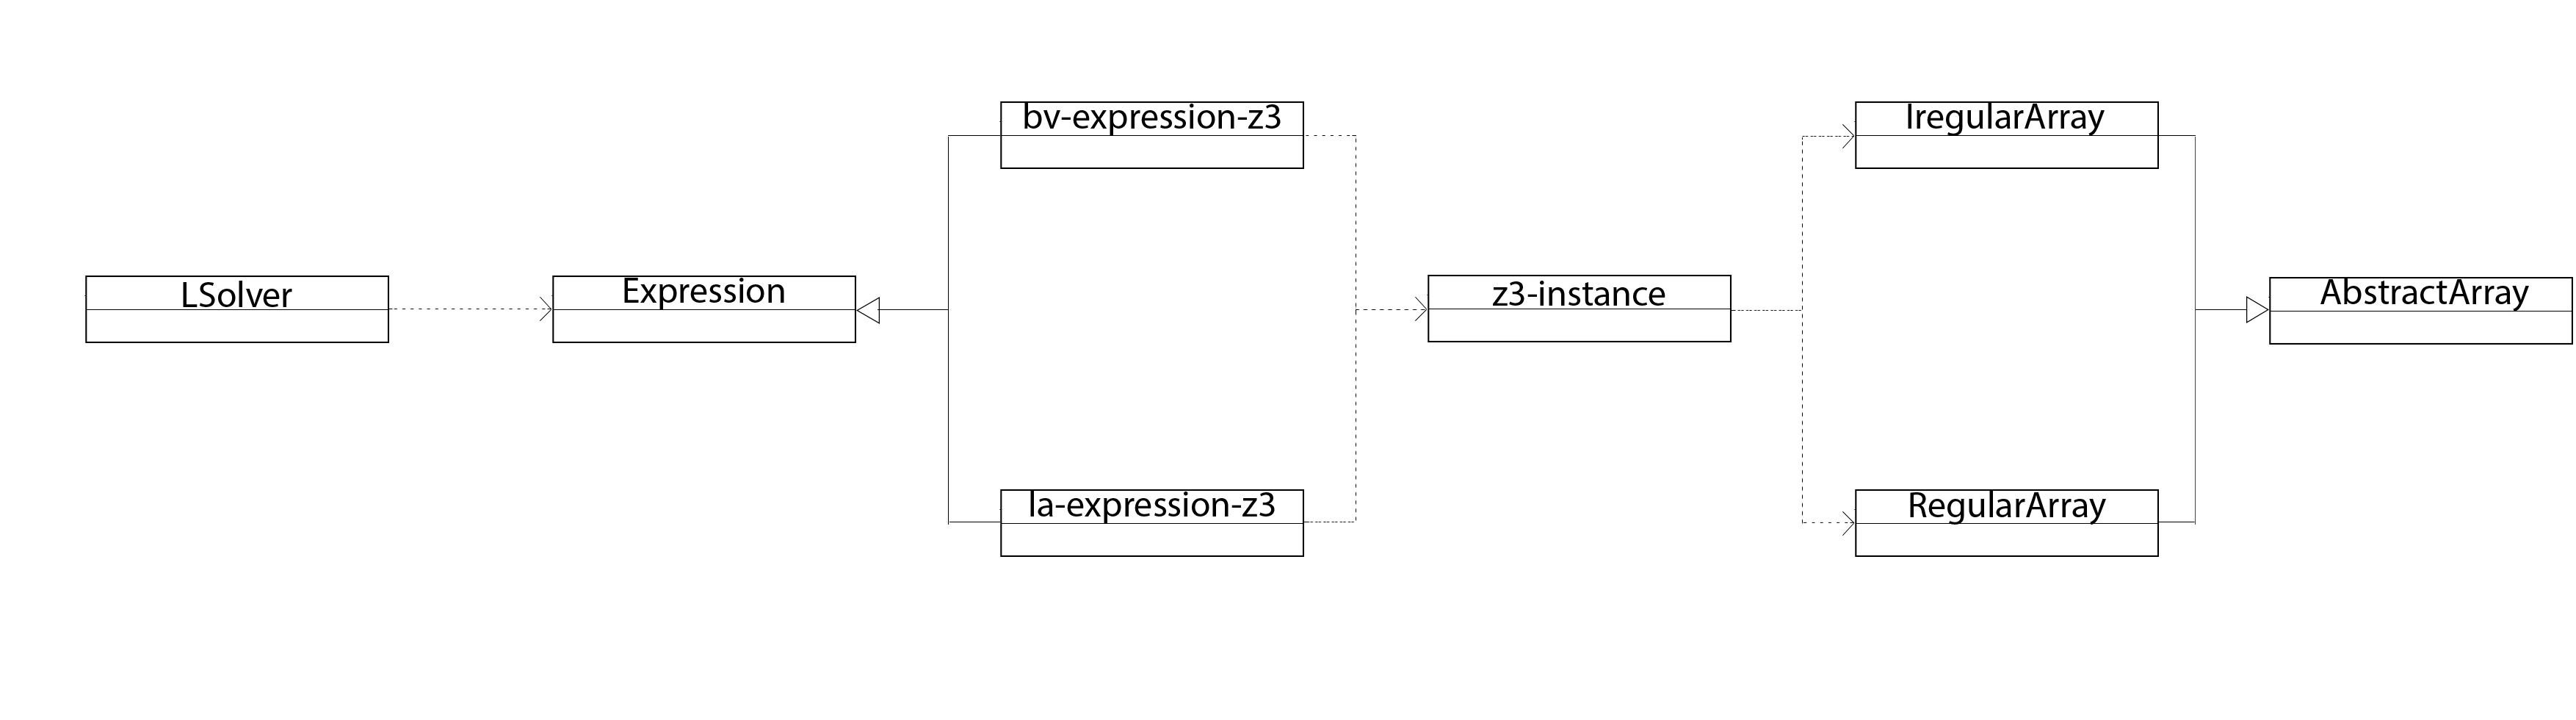
\includegraphics[width=1.2\textwidth]{dijagram.png}
  \caption{Dijagram klasa}
  \label{fig:dijagram}
\end{figure}

\par

Pri pokretanju alata LAV, opcijom \texttt{-solver=Z3-LA-ARR-EUF} označava se upotreba teorije linearne aritmetike, teorije nizova i teorije neinterpretiranih funkcija rešavača Z3. Opcijom \texttt{-solver=Z3-BV-ARR-EUF} označava se upotreba teorije bitvektora, teorije nizova i teorije neinterpretiranih funkcija rešavača Z3. Navođenjem opcije \texttt{-model} generišu se fajlovi koji sadrže vrednosti promenljivih i nizova modela nakon izvršavanja svakog bloka naredbi kao i putanja kroz program koja dovodi do greške. Za svaku potencijalno neispravnu naredbu C programa, formira se poseban fajl sa vrednostima modela. Navođenjem opcije \texttt{-test} generišu se testovi. Test primeri za koje je potrebno pokrenuti izvršavanje C programa generišu se za svaku potencijalno neispravnu naredbu programa u posebnom fajlu. Podrazumevano, test primeri se generišu u Output/test direktorijumu u okviru sistema LAV. Opcijom \texttt{-test-folder} ova putanja se može predefinisati proizvoljnom putanjom fajl sistema.

\par
\subsubsection{Automatizacija testiranja}
Automatizacija testiranja programa vrednostima modela u okviru alata LAV vrši se pokretanjem bash skripte \texttt{testiranje.sh}. Skripta izvršava ulazni C program čime se utvrđuje da li generisani test primeri dovode do nebezbednog ponašanja i softverske greške.
Kao argumenti pri pokretanju skripte navode se 
\par
\texttt{./testiranje.sh <ime\_programa> <teorija> <test\_direktorijum>}
\\ gde su:
\begin{description}
  \item \texttt{<ime\_programa>} - C program koji se testira
  \item \texttt{<teorija>} - odabir teorije u koju se formula za opisivanje ponašanja programa transformiše. Podržane teorije su teorija linearne aritmetike (navođenjem argumenta \texttt{LA}) ili teorija bitvektora (navođenjem argumenta \texttt{BV})
  \item \texttt{<test\_direktorijum>} - putanja na kojoj će se generisati test primeri u okviru fajl sistema. Ovaj argument je opcioni. Ukoliko se izostavi, podrazumevana vrednost je Output/test direktorijum u okviru sistema LAV.
\end{description}
 
Pored C programa, neophodno je postojanje još jednog C fajla
čiji naziv mora imati format \texttt{ime\_programa\_test}. Sadržaj dopunskog fajla je identičan originalnom sa dodatim anotacijama za izdvajanje naziva i tipova ulaznih promenljivih. Postoje dve vrste anotacija, uz zavisnosti da li je ulazna vrednost programa promenljiva ili niz. Za promenljive se koristi anotacija 
\texttt{input\_value(ime\_promenljive, pozici-\\ja)}, dok se za nizove koristi 
anotacija \texttt{input\_value\_array(ime\_niza, pozicija)}, gde pozicija predstavlja redni broj promenljive ili niza pri zadavanju ulaznih vrednosti. 
\par
U primeru \ref{example21} ispituje se ispravnost jednostavnog C programa korišćenjem alata LAV. Vrednosti modela rešavača ispisuju se nakon izvršavanja svakog bloka naredbi. Važno je napomenuti da generisanje modela ne zahteva uvođenje anotacija, jer nije bitan redosled nabrajanja promenljivih. 
\begin{primer} \label{example21} U ovom primeru javlja se greška pri deljenju sa nulom. Na osnovu modela, praćenjem vrednosti nakon svakog izvršenog bloka, dolazi se do putanje koja proizvodi grešku.\\
\\
\hspace{-0.6cm}
\begin{minipage}[b]{0.5\textwidth}
\textbf{C program:}\\
1  \hspace{0.1cm} \#include <stdio.h> \\ 
2  \hspace{0.1cm} int main() \{ \\
3 	\hspace{0.1cm} \tab int a, b=15;\\
4	\hspace{0.1cm} \tab scanf($"$\%d $"$, $\&$a);\\
5	\hspace{0.1cm} \tab if(a < b)\\
6	\hspace{0.1cm} \tab \tab a++;\\
7	\hspace{0.1cm} \tab if(a == b)\\
8	\hspace{0.1cm} \tab \tab b = 0;\\
9	\hspace{0.1cm} \tab return a/b;\\ 
10 \hspace{0.1cm} \}

\end{minipage}
\hspace{0.3cm}
\begin{minipage}[t]{0.4\textwidth}
\vspace{-6.65cm}
\textbf{Model:}\\
function: main\\
error: division\_by\_zero\\
9: a = 15, b = 0,\\
8: a = 15, b = 0,\\
7: a = 15, b = 15,\\
6: a = 15, b = 15,\\
5: a = 14, b = 15,
\end{minipage}
\end{primer}

U primeru \ref{example22} generiše se test primer za C program iz primera \ref{example21}. Prilikom generisanja testova, zahteva se navođenje anotacija čime se određuje redosled promenljivih u test primeru. Automatsko određivanje redosleda promenljivih programa može biti dalji pravac rada pošto je reč o netrivijalnom problemu.

\begin{primer} Test primer definisan je vrednostima modela nakon izvršene poslednje instrukcije prvog bloka. Kako je vrednost promenljive b inicijalizovana, uvodimo anotaciju samo za promenljivu a, pa test primer sadrži samo jednu vrednost. \label{example22}  
\\ \\
\hspace{-0.6cm}
\begin{minipage}[b]{0.5\textwidth}
\textbf{C program:}\\
1 \hspace{0.1cm} \#include <stdio.h> \\
2 \hspace{0.1cm} int input\_value(int, int);\\ 
3 \hspace{0.1cm} int main() \{ \\
4 \hspace{0.1cm} \tab int a, b=15;\\
5 \hspace{0.1cm} \tab scanf($"$\%d $"$, $\&$a);\\
6 \hspace{0.1cm} \tab input\_value(a,0);\\
7 \hspace{0.1cm} \tab if(a < b)\\
8 \hspace{0.1cm} \tab \tab a++;\\
9 \hspace{0.1cm} \tab if(a == b)\\
10 \hspace{0.1cm} \tab \tab b = 0;\\
11 \hspace{0.1cm} \tab return a/b;\\
12 \hspace{0.1cm} \}

\end{minipage}
\hspace{0.3cm}
\begin{minipage}[t]{0.4\textwidth}
\vspace{-7.88cm}
\textbf{Test:}\\
14
\end{minipage}
\end{primer}

U primeru 23 ispituje se ispravnost C programa koji vrši jednostavne algebarske transformacije nad elementima nizova upotrebom alata LAV. Vrednosti elemenata nizova ispisuju se nakon svakog bloka naredbi.
\begin{primer}
U ovom primeru javlja se greška pri deljenju sa nulom odgovarajućih elemenata nizova a i b. Elementi nizova kojima rešavač nije dodelio vrednosti označeni su *.\\ \\
\hspace{-0.6cm} \label{example23}
\begin{minipage}[b]{0.5\textwidth}
\textbf{C program:}\\
1 \hspace{0.1cm} \#include <stdio.h> \\
2 \hspace{0.1cm} void readInput(int array[], int n) \{ \\
3	\hspace{0.15cm} \tab int i; \\
4	\hspace{0.15cm} \tab for(i=0; i<n; i++) \\
5	\hspace{0.15cm} \tab \tab	scanf($"$\%d $"$, $\&$array[i]); \\
6 \hspace{0.1cm} \} \\
7 \hspace{0.1cm} int main()\{ \\
8	\hspace{0.15cm} \tab int a[5], b[5];\\
9	\hspace{0.15cm} \tab a[3]=0; \\
10	\hspace{-0.08cm} \tab a[4]=14; \\
11	\hspace{-0.08cm} \tab b[3]=10; \\
12	\hspace{-0.08cm} \tab b[4]=15; \\
13  \hspace{-0.08cm} \tab readInput(a, 3); \\
14  \hspace{-0.08cm} \tab readInput(b, 3); \\
15  \hspace{-0.08cm} \tab if(a[3] < b[3]) \\
16	\hspace{-0.08cm} \tab \tab	a[4]++; \\
17	\hspace{-0.08cm} \tab if(a[4] == b[4]) \\
18	\hspace{-0.08cm} \tab \tab	b[4]=0; \\
19	\hspace{-0.08cm} \tab return a[4]/b[4]; \\
20 \}
\end{minipage}
\hspace{1.1cm}
\begin{minipage}[t]{0.4\textwidth}
\vspace{-12.98cm}
\textbf{Model:}\\
function: main \\
error: division\_by\_zero \\
19: a[] = \{*, *, *, 0, 15\}, \\ b[] = \{*, *, *, 10, 0\} \\ \\
18: a[] = \{*, *, *, 0, 15\}, \\ b[] = \{*, *, *, 10, 0\} \\ \\
17: a[] = \{*, *, *, 0, 15\}, \\ b[] = \{*, *, *, 10, 15\} \\ \\
16:	a[] = \{*, *, *, 0, 15\}, \\ b[] = \{*, *, *, 10, 15\} \\ \\
15: a[] = \{*, *, *, 0, 14\}, \\ b[] = \{*, *, *, 10, 15\}
\end{minipage}
\end{primer} 
\par
U primeru \ref{example24} generiše se test primer za C program iz primera \ref{example23}. Navode se anotacije kojima se određuje redosled učitavanja odgovarajućih elemenata nizova.
 
\begin{primer} Generisani test primer odgovara vrednostima modela rešavača nakon izvršenog prvog bloka naredbi. Kako su vrednosti četvrtog i petog elementa nizova a i b inicijalizovane, test primer sadrži samo vrednosti koje učitavamo korišćenjem funkcije \texttt{scanf}. Test vrednosti za elemente nizova kojima rešavač nije dodelio vrednosti označene su 1.\\ \\
\hspace{-0.6cm} \label{example24}
\begin{minipage}[b]{0.5\textwidth}
\textbf{C program:}\\
1 \hspace{0.1cm} \#include <stdio.h> \\
2 \hspace{0.1cm} void readInput(int array[], int n) \{ \\
3	\hspace{0.15cm} \tab int i; \\
4	\hspace{0.15cm} \tab for(i=0; i<n; i++) \\
5	\hspace{0.15cm} \tab \tab	scanf($"$\%d $"$, $\&$array[i]); \\
6 \hspace{0.1cm} \} \\
7 \hspace{0.1cm} int main()\{ \\
8	\hspace{0.15cm} \tab int a[5], b[5];\\
9	\hspace{0.15cm} \tab a[3]=0; \\
10	\hspace{-0.08cm} \tab a[4]=14; \\
11	\hspace{-0.08cm} \tab b[3]=10; \\
12	\hspace{-0.08cm} \tab b[4]=15; \\
13  \hspace{-0.08cm} \tab readInput(a, 3); \\
14  \hspace{-0.08cm} \tab readInput(b, 3); \\
15	\hspace{-0.08cm} \tab input\_value\_array(a, 0); \\
16	\hspace{-0.08cm} \tab input\_value\_array(b, 1); \\
17  \hspace{-0.08cm} \tab if(a[3] < b[3]) \\
18	\hspace{-0.08cm} \tab \tab	a[4]++; \\
19	\hspace{-0.08cm} \tab if(a[4] == b[4]) \\
20	\hspace{-0.08cm} \tab \tab	b[4]=0; \\
21	\hspace{-0.08cm} \tab return a[4]/b[4]; \\
22 \}
\end{minipage}
\hspace{1.1cm}
\begin{minipage}[t]{0.4\textwidth}
\vspace{-14.2cm}
\textbf{Test:}\\
1 1 1 1 1 1
\end{minipage}
\end{primer}



% ------------------------------------------------------------------------------
\chapter{Zaključak} \label{zakljucak}
U ovom radu razmatran je problem ispitivanja ispravnosti softvera korišćenjem tehnika statičke automatizovane analize. 
Uslovi neispravnosti programa definisani su formulama u terminima matematičkih teorija. Modeli ovih formula se mogu koristiti za automatsko generisanje test primera za koje se proverava da li zaista dovode do greške u softveru.
\par
Alatu LAV dodata je podrška za preciznije izdvajanje modela u radu sa Z3 rešavačem
koji pokriva različite kombinacije teorija. Podržane teorije, kojima je moguće modelovati uslove ispravnosti programa, su teorija neinterpretiranih funkcija, teorija linearne aritmetike,
teorija bitvektora i teorija nizova.

Prilikom pravljenja modela ponašanja programa, korišćenjem izabrane teorije,
primenjuju se razne aproksimacije. 
Zbog ovih aproksimacija, mogu se prijaviti greške u programu koje zapravo ne postoje. Iz tog razloga neophodno je pokretanjem
programa proveriti da li generisani test primer stvarno dovodi do nebezbednog i
neočekivanog ponašanja. Alatu LAV dodata je podrška za automatsko
generisanje test primera na osnovu vrednosti iz modela rešavača Z3 za izabranu
teoriju.
 
Eksperimentalni rezultati koji ukazuju na bolje performanse pri korišćenju rešavača Z3 u poređenju sa drugim SMT rešavačima dostupni su u literaturi \cite{z3improvements}. U radu je detaljno opisana upotreba rešavača korišćenjem SMT-LIB standarda i C++ interfejsa.

Buduća istraživanja na temu unapređenja rada mogla bi da obuhvate automatsko određivanje ulaznih promenljivih, da bi se izbeglo dodatno anotiranje promenljivih u samom kodu. Drugo unapređenje moglo bi da obuhvati preciznije izdvajanje modela za druge SMT rešavače pokrivanjem različitih kombinacija teorija. Takođe, format ispisa vrednosti modela i test primera za sve rešavače mogao bi se standardizovati. 
% ------------------------------------------------------------------------------


% ------------------------------------------------------------------------------
% Literatura
% ------------------------------------------------------------------------------
\literatura

% ==============================================================================
% Završni deo teze i prilozi
\backmatter
% ==============================================================================

% ------------------------------------------------------------------------------ ------------------------------------------------------------------------------

\end{document}
